%% =====================================================================
%%  CloudSim Plus-K8s: A Contract-Driven Extension for
%%  Kubernetes Container Orchestration Simulation
%%
%%  Source:        kubernetes-cloudsimplus.tex
%%  Bibliography:  kubernetes-refs.bib
%%
%%  Compilation (Overleaf or local TeX Live with USG.cls available):
%%      pdflatex kubernetes-cloudsimplus
%%      bibtex   kubernetes-cloudsimplus
%%      pdflatex kubernetes-cloudsimplus
%%      pdflatex kubernetes-cloudsimplus
%% =====================================================================

\documentclass[ASNA,twocolumn]{USG}

% ------------------------------------------------------------ packages
\usepackage{anyfontsize}
\usepackage{colortbl}
\usepackage{xcolor}
\usepackage{booktabs}
\usepackage{tabularx}
\usepackage{threeparttable}
\usepackage{mathtools}
\usepackage{bm}
\usepackage{tikz}
\usetikzlibrary{arrows.meta,positioning,shapes.geometric,fit,calc,backgrounds}
\usepackage{algorithm}
\usepackage{algpseudocode}
\usepackage{enumitem}
\setlist{nosep}
\usepackage{xspace}

\graphicspath{{./images/}}

% ----- Submission-ready: \todomark is defined but suppressed.
\newcommand{\todomark}[1]{}

% ----- Convenience commands ------------------------------------------
\newcommand{\ckm}{CloudSim Plus-K8s\xspace}

% ============================== Document ==============================
\articletype{ORIGINAL ARTICLE}
\journal{Software: Practice and Experience}
\volume{0}
\copyyear{2026}
\startpage{1}
\articledoi{10.1002/spe.0000}

% Submission-history placeholders (filled in by the journal at production).
\received{00 Month 2026}
\revised{00 Month 2026}
\accepted{00 Month 2026}

\begin{document}
    \title{CloudSim Plus-K8s: A Contract-Driven Extension for Kubernetes Container Orchestration Simulation}

    \author[1]{Zarai Othmane}

    \author[1]{Ettazi Widad}
    
    \author[1]{Riane Driss}

    \authormark{ZARAI \textsc{and} ETTAZI}
    \titlemark{CLOUDSIM PLUS-K8S: KUBERNETES ORCHESTRATION SIMULATION}

    \address[1]{\orgdiv{IMS Team-ADMIR Laboratory ENSIAS-Rabat IT Center}, \orgname{Mohammed V University in Rabat}, \orgaddress{\state{Rabat}, \country{Morocco}}}

    \corres{Othmane Zarai (\email{othmane\_zarai@um5.ac.ma})}
    

    \keywords{CloudSim Plus | Kubernetes | pod scheduling | horizontal/vertical pod autoscaling | cluster autoscaler | M/M/c queueing | Jaeger distributed tracing | sim-to-real validation}

    \abstract[ABSTRACT]{
    We present CloudSim Plus-K8s, a discrete-event simulation extension of CloudSim Plus that models Kubernetes scheduling (filtering and scoring), horizontal and vertical autoscaling, workload controllers, and per-service microservice latency under an explicit, testable fidelity contract enforced by a validation suite comprising 214 tests. Validated against a four-node Oracle Cloud k3s cluster running Google's Online Boutique, the simulator achieves 100\% filter and feasibility agreement with kube-scheduler on both a 300-scenario synthetic benchmark and the live cluster, while reproducing the steady-state behaviour of every modelled controller exactly (zero steady-state replica error). Compared with the official kube-scheduler-simulator on a cluster substrate matched to the simulator's, strict winner-node agreement reaches 84\% (5-run mean; range 82--87\%). Across all 300 scenarios, the kube-scheduler winner is contained within the simulator's tied minimum-score set, yielding 100\% combined agreement on both the synthetic and live substrates. The remaining strict disagreement arises solely from deterministic versus random tie-breaking among co-optimal nodes rather than from filtering failures or scoring-policy differences; re-running all 300 scenarios under a matched least-allocated profile does not change any placements. A trace-driven Online Boutique study characterises the operating regime of the analytic M/M/c latency model. The model reproduces traced per-operation $p95$ latency within $\pm0.5 \log_{10}$ for one of eight operations under moderate load, with accuracy degrading under saturation as the model's open-system assumptions no longer hold. Rather than claiming general fidelity, we provide a falsifiable specification of the Kubernetes behaviours reproduced by the simulator and their associated tolerances, together with an open-source, reproducible artifact.
    }

    \abbr{HPA, Horizontal Pod Autoscaler; VPA, Vertical Pod Autoscaler;
    CA, Cluster Autoscaler; DES, Discrete-Event Simulation;
    MIPS, Million Instructions Per Second; PE, Processing Element;
    QoS, Quality of Service; SLA, Service Level Agreement;
    CNCF, Cloud Native Computing Foundation; DAG, Directed Acyclic Graph;
    NRMSD, Normalised Root-Mean-Square Deviation.}

    \maketitle

%%============================================================
    \section{Introduction}\label{sec:intro}
%%============================================================

    Kubernetes~\cite{Burns2016,Verma2015} has established itself as the
    dominant platform for container orchestration in production cloud environments. According to the Cloud Native Computing Foundation (CNCF) Annual Survey, 84\% of respondents are using or evaluating Kubernetes, with 66\% running it in production~\cite{CNCF2023}. The platform's success is attributable to its rich set of abstractions pods,
    services, deployments, namespaces and its sophisticated scheduling
    and autoscaling machinery that collectively realise the promise of
    self-healing, elastic, and observable distributed applications.
    Kubernetes scheduling has consequently attracted substantial research
    attention: surveys catalogue dozens of optimisation approaches spanning
    heuristic, constraint-based, and learning-driven
    methods~\cite{Li2023}, and reinforcement learning schedulers
    demonstrably outperform the default kube-scheduler on real-world
    heterogeneous workloads~\cite{Xie2024}.

    Our prior systematic review of intelligent autoscaling strategies for
    cloud-native microservices~\cite{Zarai2025} identified three recurring
    blockers to deployable autoscaling research: (i)~the \emph{sim-to-real
    gap}, where agents trained or tuned in idealised environments fail to
    transfer to production clusters; (ii)~the absence of \emph{standardised
    testing frameworks}, which limits cross-study reproducibility and
    generalisation; and (iii)~limited \emph{real-world deployment evidence}
    behind reported gains. The work presented in this paper targets the
    first two of these blockers directly: it provides a high-fidelity,
    reproducible simulation substrate in which novel scheduling and
    autoscaling algorithms can be evaluated under identical workload traces
    \emph{before} paying the cost of a real cluster, while preserving the
    semantic fidelity required for results to transfer.
    
    The need for simulation in cloud computing research is well
    established. Real cloud deployments are prohibitively expensive for
    exhaustive algorithmic evaluation, and reproducibility is often
    compromised by dynamic pricing, ephemeral infrastructure, and
    non-deterministic workload co-location~\cite{Calheiros2011,Pucher2015}.
    Discrete-event simulation (DES) frameworks such as
    CloudSim~\cite{Calheiros2011} and its successor CloudSim Plus~\cite{Silva2017} provide controlled, repeatable environments in
    which researchers can evaluate scheduling policies, resource provisioning strategies, and energy management algorithms at scale,
    with the ability to replay real workload traces such as the Google Cluster Traces~\cite{Bappy2023} and PlanetLab CPU utilisation records.

    However, a significant semantic gap persists between what current
    simulators model and what Kubernetes provides. Existing
    extensions including ContainerCloudSim~\cite{Piraghaj2017},
    CloudNativeSim~\cite{Wu2025}, and CloudSim 7G~\cite{Andreoli2025} address
    specific aspects of container and microservice simulation but stop
    short of providing a high-fidelity model of the full Kubernetes
    orchestration stack: its label-selector-based pod routing, its
    multi-pass filter-and-score scheduler, its declarative workload
    controllers, and its reactive autoscaling subsystems. Specialised tools
    such as K8sSim~\cite{Wen2023} and the official kube scheduler
    simulator~\cite{KubeSchSim2025} focus on scheduling decision replay but
    provide no lifecycle, controller, or autoscaling simulation.

    CloudSim Plus provides an architecturally mature foundation for such an
    extension. Its sealed-interface hierarchy, null-object pattern,
    pluggable strategy implementations, and topology-aware allocation
    policies provide the composability required to layer Kubernetes
    semantics atop a proven DES engine without modifying core framework code.

    This paper makes four main contributions:
    (i)~a systematic entity mapping and a composition architecture
    that layers Kubernetes semantics over the CloudSim Plus core with a
    minimal core footprint --- one small \texttt{DatacenterSimple} edit
    plus \texttt{module-info} exports, no changes to core scheduling or
    allocation logic;
    (ii)~a three-stage filter-and-score scheduler with eviction-style
    preemption, tick-driven control plane (six workload controllers,
    controller manager, kubelet), and high-fidelity HPA/VPA/Cluster
    Autoscaler --- together with networking, storage, and security
    primitives;
    (iii)~a fifteen-example worked-example suite and a deployment kit driving a
    sim-to-real validation against an Oracle Cloud k3s cluster, with a
    paired Online Boutique trace-comparison track; and
    (iv)~an explicit, test-enforced simplifications contract
    mapped one-to-one to regression
    tests. 
    The Kubernetes extension source lives in a public development fork of
    CloudSim Plus; the fork URL and reproducibility artefacts are given in
    the Data Availability Statement.%

    The remainder of the paper is organised as follows.
    Section~\ref{sec:background} reviews CloudSim Plus and
    Kubernetes; Section~\ref{sec:related} surveys related tools;
    Section~\ref{sec:architecture} presents the framework architecture;
    Sections~\ref{sec:scheduling}--\ref{sec:autoscaling} detail the
    scheduling, control-plane, and autoscaling subsystems;
    Section~\ref{sec:validation} reports the validation methodology and
    empirical results; Section~\ref{sec:examples} walks through the worked
    examples; Section~\ref{sec:zarai-mapping} discusses how \ckm maps onto
    the open challenges identified in our prior systematic review; and
    Section~\ref{sec:conclusions} concludes.

%%============================================================
    \section{Background}\label{sec:background}
%%============================================================

    \subsection{CloudSim Plus}

    CloudSim Plus~\cite{Silva2017} is a modern Java-based DES framework
    for modelling cloud computing infrastructures, reengineered from the
    original CloudSim~\cite{Calheiros2011} with an emphasis on software
    engineering principles: interface-driven design with sealed hierarchies,
    the null-object pattern for safe absent-entity handling, pluggable
    strategy implementations for schedulers and allocation policies, and
    fluent builder APIs.

    The simulation engine advances a discrete clock to successive event
    times, dispatching \texttt{SimEvent} messages among \texttt{SimEntity}
    participants. The principal entity hierarchy is \texttt{Datacenter}
    $\supset$ \texttt{Host} $\supset$ \texttt{Vm} $\supset$ \texttt{Cloudlet},
    corresponding to the physical-to-logical nesting of a cloud datacenter.
    Resource provisioning is governed by pluggable \texttt{ResourceProvisioner}
    implementations; VM placement is handled by \texttt{VmAllocationPolicy}
    implementations; and cloudlet execution within VMs is governed by
    \texttt{CloudletScheduler} implementations.

    As the allocation substrate for the Kubernetes layer, \emph{this
    work} contributes a topology-aware host and allocation policy
    (\texttt{TopologyAwareHost} and
    \texttt{VmAllocationPolicyTopologyAware}) to the CloudSim Plus core
    packages. The policy extends the stock
    \texttt{VmAllocationPolicyAbstract}; it models multi-tier datacenter
    topology (racks, zones, regions) and applies cost, latency, or spread
    objectives during VM placement. This substrate forms the direct
    foundation upon which the Kubernetes layer is built; it is part of the
    same contribution and is \emph{not} present in any released upstream
    CloudSim Plus version (the latest public release is~8.5.7; the code
    currently lives in a public development fork. 
    CloudSim Plus has also inspired several domain-specific extensions,
    including PureEdgeSim~\cite{PureEdgeSim} for IoT/edge simulation
    (supporting 30{,}000+ devices and 24+ hour simulations), confirming
    its suitability as a general-purpose cloud-native simulation base.

    \subsection{Kubernetes Architecture}

    Kubernetes~\cite{Verma2015,Burns2016} is a distributed container
    orchestration system designed in the lineage of Google's
    Borg~\cite{Verma2015}, with which it shares several core design
    principles. Its architecture separates control-plane and
    data-plane responsibilities. The \emph{control plane} comprises the
    API server, the \emph{kube-scheduler} (pod-to-node assignment), the
    \emph{controller manager} (workload reconciliation), and \emph{etcd}
    (distributed key-value store). The \emph{data plane} consists of
    worker nodes, each running a \emph{kubelet} (local reconciliation
    agent) and a container runtime.

    Kubernetes models workloads as \emph{pods}---the minimal schedulable
    unit comprising one or more co-located containers. Pods carry metadata
    labels; the scheduler and controllers use \emph{label selectors} to
    identify pod groups. Nodes carry labels and may carry \emph{taints};
    pods declare \emph{tolerations} to overcome taint-based exclusions and
    \emph{node affinity} rules to express placement preferences.

    The scheduler implements a two-phase algorithm: a \emph{filter} phase
    eliminates nodes that violate hard constraints (resource capacity,
    nodeSelector, node affinity, taints/tolerations, required pod affinity
    rules), followed by a \emph{score} phase that ranks feasible nodes by
    soft preferences (preferred node affinity weights, pod
    affinity/anti-affinity bonuses, resource balance scores). Six workload
    controller types govern pod lifecycle at the fleet level: Deployment
    (stateless, rolling updates), ReplicaSet (replica maintenance),
    StatefulSet (stable identities), Job (batch completion), CronJob
    (scheduled batch), and DaemonSet (one-per-node). The Horizontal Pod
    Autoscaler adjusts replica counts in response to resource utilisation,
    while the Cluster Autoscaler provisions or decommissions nodes in
    response to scheduling pressure.

%%============================================================
    \section{Related Work}\label{sec:related}
%%============================================================

    Prior simulation support for containerised and orchestrated workloads
    falls into two broad families, and we organise the survey accordingly.
    The first --- \emph{cloud simulation frameworks for containerized
    environments} (Section~\ref{sec:related-frameworks}) --- extends
    general-purpose cloud discrete-event simulators (CloudSim and its
    descendants, iFogSim) with containers, microservice call graphs,
    auto-scaling loops, or serverless functions, but stops short of
    modelling the Kubernetes orchestration semantics. The second ---
    \emph{Kubernetes-specific simulation and evaluation tools}
    (Section~\ref{sec:related-k8s}) --- targets Kubernetes directly, but
    each existing tool covers only a slice of the stack (the scheduler, or
    the autoscalers, or the service-call graph) rather than the scheduler,
    controllers, lifecycle, and autoscalers together.
    Section~\ref{sec:related-gap} then draws the capability comparison
    (Table~\ref{tab:comparison}) that positions \ckm against both families.

    \subsection{Cloud Simulation Frameworks for Containerized Environments}
    \label{sec:related-frameworks}

    This family adapts general-purpose cloud simulators to container-,
    microservice-, or serverless-level workloads; none models the
    Kubernetes control plane. We summarise each tool below and note the
    Kubernetes-specific constructs it leaves unaddressed.

    Fotuhi Piraghaj et al.~\cite{Piraghaj2017} proposed ContainerCloudSim,
    extending CloudSim 3.x with support for containers co-located within
    VMs, enabling study of container placement and consolidation under SLA
    and energy constraints. ContainerCloudSim models two-layer
    virtualisation (VMs inside hosts, containers inside VMs) and supports
    container migration with startup delays. It does not model
    Kubernetes-specific constructs such as label selectors, pod affinity,
    taints/tolerations, or workload controllers, and its container
    abstraction does not distinguish init containers from main containers.

    Andreoli et al.~\cite{Andreoli2025} re-engineered the CloudSim
    ecosystem in CloudSim 7G, introducing unified
    \texttt{HostEntity}/\texttt{GuestEntity} interfaces that generalise
    VMs, containers, and nested entities. The redesign reduces code
    duplication significantly and enables seamless integration of
    NetworkCloudSim and ContainerCloudSim modules. CloudSim 7G provides
    structural foundations for containers running in nodes, but lacks the
    semantic Kubernetes layer: no label-selector matching, no
    affinity/taint model, and no Kubernetes-style workload controllers.

    Wu et al.~\cite{Wu2025} built CloudNativeSim on CloudSim 3.0 to
    simulate cloud-native microservice applications. It introduces
    DAG-based service dependency graphs, per-instance replica modelling,
    and QoS tracking with Grafana integration, achieving 94.5\% accuracy
    in response-time simulation. CloudNativeSim focuses on inter-service
    communication latency and throughput metrics; it does not model
    Kubernetes scheduler semantics (node affinity, taints, pod affinity),
    workload controllers, or autoscaling.

    Aslanpour et al.~\cite{Aslanpour2021} proposed AutoScaleSim, extending
    CloudSim with a MAPE-K (Monitor, Analyse, Plan, Execute) loop for
    web-application auto-scaling. AutoScaleSim models VM startup delays
    and measures 20+ performance metrics, with validation against
    OpenStack. While conceptually aligned with HPA behaviour, AutoScaleSim
    operates at the VM level rather than the pod level and does not
    incorporate Kubernetes control-plane machinery or cluster-level
    autoscaling.

    Mahmud et al.~\cite{Mahmud2021} presented iFogSim2, extending iFogSim
    with mobility, clustering, and microservice management modules for
    edge/fog environments. The microservice component orchestrates service
    replicas across federated multi-tier nodes. While modelling
    inter-service dependencies and basic replica management, iFogSim2's
    placement policies are simplified compared to the full Kubernetes
    scheduling model, and it does not implement declarative controller
    reconciliation loops.

    Mahmoudi and Khazaei~\cite{Mahmoudi2021} presented SimFaaS for
    serverless function-as-a-service simulation, bridging Markovian
    performance models with practical simulation environments. SimFaaS
    focuses on cold-start and scaling dynamics specific to FaaS platforms,
    a domain orthogonal to but complementary with Kubernetes pod-based
    orchestration.

    \subsection{Kubernetes-Specific Simulation and Evaluation Tools}
    \label{sec:related-k8s}

    This family models Kubernetes constructs directly rather than adapting
    a general cloud simulator. Each tool is high-fidelity within its chosen
    slice of the stack --- scheduling decisions, autoscaling loops, or the
    service-call graph --- but narrower in scope than a full orchestration
    model, as the closing comparison makes explicit.

    Wen et al.~\cite{Wen2023} proposed K8sSim, the first simulator
    specifically targeting Kubernetes scheduling algorithm evaluation. By
    replaying scheduling decisions without running a live cluster, K8sSim
    achieves a 38.56$\times$ speedup over real-cluster evaluation and
    benchmarks 11 Kubernetes and 13 Volcano scheduling algorithms against
    real Alibaba cluster traces. However, K8sSim evaluates placement
    decisions only; it does not simulate pod lifecycle, workload
    controllers, or autoscaling subsystems, making it complementary to
    but narrower in scope than \ckm.

    The Kubernetes project itself publicised the
    \texttt{kube-scheduler-simulator}~\cite{KubeSchSim2025} in an April 2025
    Kubernetes blog post; it is an official tool that wraps the production (debuggable)
    \texttt{kube-scheduler} and replays scheduling decisions against a
    synthetic cluster state. It does \emph{not} require a live cluster:
    it runs the scheduler and a \texttt{kube-apiserver} over a
    KWOK-backed fake cluster (Kubernetes WithOut Kubelet) in Docker, so
    nodes and pods are simulated objects rather than real workloads.
    While this guarantees exact algorithmic fidelity (it executes
    production scheduling code), it is not a DES framework: it reproduces
    scheduling \emph{decisions} exactly but does not model datacenter
    topology, resource-utilisation dynamics, or autoscaler interactions
    within a single controlled experiment.

    Skenario~\cite{Skenario} provides a discrete-event simulation of
    Kubernetes HPA and VPA autoscaling control loops in isolation,
    offering a web UI for testing scaling policies with synthetic traffic
    profiles. It does not model the pod scheduler, workload controllers,
    or container lifecycle.

    Two recent efforts target the orchestration-simulation and
    digital-twin space directly. \emph{Kubernetes-in-the-Loop}
    (Straesser et al.~\cite{Straesser2023}) makes the opposite substrate
    choice to ours: rather than simulating the control plane, it embeds a
    \emph{real} Kubernetes control plane in the loop of a microservice
    performance simulation, so scheduling and scaling are executed by
    authentic Kubernetes while workload and service times are simulated.
    This yields high orchestration fidelity but reintroduces the cluster
    dependency and run-to-run non-determinism that a pure DES avoids.
    \emph{KubeTwin} (Borsatti et al.~\cite{Borsatti2024}) builds a digital
    twin of large-scale Kubernetes deployments for performance prediction
    and what-if analysis; like \ckm it is simulation-based and
    scale-oriented, but it is calibrated as a deployment-specific twin
    rather than a general, contract-documented model of the orchestration
    stack with a published simplifications list.

    These tools differ from \ckm along three axes. \emph{Scope}:
    K8sSim and \texttt{kube-scheduler-simulator} cover the scheduler only,
    Skenario the autoscalers only, CloudNativeSim the service-call graph,
    whereas \ckm models scheduler, controllers, lifecycle, and
    autoscalers together. \emph{Fidelity mechanism}: K8sSim replays and
    \texttt{kube-scheduler-simulator}/Kubernetes-in-the-Loop \emph{execute}
    production code (exact but cluster- or binary-bound), CloudNativeSim
    reports $>94.5\%$ response-time accuracy on its DAG model, whereas
    \ckm trades exactness for a documented, test-enforced DES contract.
    \emph{Substrate}: live or KWOK-backed fake clusters and a real control
    plane respectively, versus a pure CloudSim Plus DES engine that needs
    no cluster at all. These tools are therefore complementary to, not
    subsumed by, \ckm.

    \subsection{Gap Analysis}
    \label{sec:related-gap}

    Table~\ref{tab:comparison} compares \ckm with the
    surveyed tools across key capability dimensions. No existing
    simulator comprehensively models Kubernetes scheduling semantics,
    declarative workload controllers, pod lifecycle management, and
    autoscaling subsystems simultaneously. \ckm addresses
    this gap while retaining full compatibility with the CloudSim Plus core.

    \begin{table*}[tp]
        \centering
        \caption{Comparison of container and orchestration simulation
        frameworks. \checkmark~= Supported; $\times$~= Not supported;
        $\sim$~= Partial support. CS = CloudSim version; CSP = CloudSim
        Plus.\label{tab:comparison}}
        \begin{threeparttable}
            \begin{tabular*}{\textwidth}{@{\extracolsep{\fill}}lccccccc@{}}
\toprule
\textbf{Feature} & \textbf{CCS\tnote{a}} & \textbf{CS7G\tnote{b}} & \textbf{CNS\tnote{c}} & \textbf{ASS\tnote{d}} & \textbf{iFog2\tnote{e}} & \textbf{K8sSim\tnote{f}} & \textbf{Ours} \\
\midrule
Label / Selector Matching      & $\times$ & $\times$ & $\times$ & $\times$ & $\times$ & $\times$ & \checkmark \\
Node Affinity                  & $\times$ & $\times$ & $\times$ & $\times$ & $\times$ & $\times$ & \checkmark \\
Pod Affinity / Anti-affinity   & $\times$ & $\times$ & $\times$ & $\times$ & $\times$ & $\times$ & \checkmark \\
Taints and Tolerations         & $\times$ & $\times$ & $\times$ & $\times$ & $\times$ & $\times$ & \checkmark \\
Declarative Controllers        & $\times$ & $\times$ & $\sim$   & $\times$ & $\sim$   & $\times$ & \checkmark \\
Init Containers                & $\times$ & $\times$ & $\times$ & $\times$ & $\times$ & $\times$ & \checkmark \\
Health Probes                  & $\times$ & $\times$ & $\times$ & $\sim$   & $\times$ & $\times$ & \checkmark \\
Horizontal Pod Autoscaler      & $\times$ & $\times$ & $\times$ & $\sim$   & $\times$ & $\times$ & \checkmark \\
Vertical Pod Autoscaler        & $\times$ & $\times$ & $\times$ & $\sim$   & $\times$ & $\times$ & \checkmark \\
Cluster Autoscaler             & $\times$ & $\times$ & $\times$ & $\sim$   & $\times$ & $\times$ & \checkmark \\
NetworkPolicy / Ingress        & $\times$ & $\times$ & $\sim$   & $\times$ & $\times$ & $\times$ & \checkmark \\
Persistent Volumes             & $\times$ & $\sim$   & $\times$ & $\times$ & $\times$ & $\times$ & \checkmark \\
ConfigMap / Secret / RBAC      & $\times$ & $\times$ & $\times$ & $\times$ & $\times$ & $\times$ & \checkmark \\
Realistic Trace Support        & $\times$ & $\times$ & $\times$ & $\times$ & $\times$ & \checkmark & \checkmark \\
Base Framework                 & CS3      & CS7G     & CS3      & CS3      & CS5      & custom    & CSP        \\
\bottomrule
            \end{tabular*}
            \begin{tablenotes}\footnotesize
                \item[a] ContainerCloudSim~\cite{Piraghaj2017}.
                \item[b] CloudSim 7G~\cite{Andreoli2025}.
                \item[c] CloudNativeSim~\cite{Wu2025}.
                \item[d] AutoScaleSim~\cite{Aslanpour2021}.
                \item[e] iFogSim2~\cite{Mahmud2021}.
                \item[f] K8sSim~\cite{Wen2023}.
            \end{tablenotes}
        \end{threeparttable}
    \end{table*}

%%============================================================
    \section{Framework Architecture}\label{sec:architecture}
%%============================================================

    \subsection{Design Principles}

    \ckm was designed around three principles. First,
    \emph{composition with a minimal core footprint}: the Kubernetes
    layer comprises 63 source files that extend stock CloudSim Plus
    classes (\texttt{VmSimple}, \texttt{CloudletSimple},
    \texttt{DatacenterBrokerSimple}) or the topology substrate this work
    adds (\texttt{TopologyAwareHost},
    \texttt{VmAllocationPolicyTopologyAware}); no core scheduling or
    allocation \emph{logic} is altered. The only edits to pre-existing
    core files are a one-line change in \texttt{DatacenterSimple} ---
    wrapping the host list in a mutable collection so the Cluster
    Autoscaler can add and remove hosts at runtime --- and the
    corresponding \texttt{module-info} package exports. This
    low-footprint structure eases forward compatibility with
    future CloudSim Plus releases. Given identical
    seeds and identical workload inputs, two \ckm runs produce
    bit-identical event timelines; the only nondeterminism surface is
    the tie-break strategy (Section~\ref{sec:tie-break}). All classes
    carry GPLv3 licence headers, use Lombok consistently, respect the
    30-statement method limit enforced by Checkstyle, and provide
    null-object constants following the framework null-object pattern.

    Second, \emph{semantic fidelity}: wherever possible, Kubernetes
    behaviour is preserved exactly---including the specific semantics of
    label-selector expressions, the topology-key scoping of pod
    affinity, and the distinction between \texttt{NO\_SCHEDULE} and
    \texttt{NO\_EXECUTE} taint effects. This fidelity is essential for
    generating simulation results that transfer to real deployments.

    Third, \emph{leverage existing infrastructure}: rather than
    reimplementing topology awareness, \ckm extends the existing
    topology-aware allocation policy and host, reusing the
    rack/zone/region model as the topology substrate for pod affinity
    topology keys.

    \subsection{Entity Mapping}

    Table~\ref{tab:mapping} presents the entity mapping from Kubernetes
    concepts to \ckm classes. The mapping is guided by the
    principle of minimal representation: a Kubernetes \emph{pod} is the
    schedulable unit, analogous to a CloudSim Plus \emph{Vm}; a
    \emph{container} is the execution unit, analogous to a
    \emph{Cloudlet}; and a \emph{node} is the physical execution substrate,
    analogous to a \emph{Host}.

    \begin{table*}[tp]
        \centering
        \caption{Kubernetes-to-\ckm entity mapping.\label{tab:mapping}}
        \small
        \setlength{\extrarowheight}{0pt}%
        \renewcommand{\arraystretch}{0.86}%
        \begin{tabular*}{\textwidth}{@{\extracolsep{\fill}}lll@{}}
\toprule
\textbf{Kubernetes Concept} & \textbf{\ckm Class} & \textbf{Superclass} \\
\midrule
Pod                    & \texttt{KubernetesPod}              & \texttt{VmSimple} \\
Container              & \texttt{KubernetesContainer}        & \texttt{CloudletSimple} \\
Node                   & \texttt{KubernetesNode}             & \texttt{TopologyAwareHost} \\
Namespace              & \texttt{Namespace}                  & --- \\
Service                & \texttt{KubernetesService}          & --- \\
Scheduler              & \texttt{KubernetesScheduler}        & \texttt{VmAllocationPolicyTopologyAware} \\
Control Plane / Broker & \texttt{KubernetesClusterBroker}    & \texttt{DatacenterBrokerSimple} \\
Labels                 & \texttt{LabelSet}                   & --- \\
Label Selector         & \texttt{LabelSelector}              & --- \\
Node Affinity          & \texttt{NodeAffinity}               & --- \\
Pod Affinity           & \texttt{PodAffinity}                & --- \\
Taint                  & \texttt{Taint} (record)             & --- \\
Toleration             & \texttt{Toleration} (record)        & --- \\
Resource Requests/Limits & \texttt{Resources} (record)       & --- \\
Pod Phase              & \texttt{PodPhase} (enum)            & --- \\
Pod Condition          & \texttt{PodCondition} (enum)        & --- \\
Deployment             & \texttt{DeploymentController}       & \texttt{ReplicaSetController} \\
ReplicaSet             & \texttt{ReplicaSetController}       & \texttt{Controller} \\
StatefulSet            & \texttt{StatefulSetController}      & \texttt{ReplicaSetController} \\
Job                    & \texttt{JobController}              & \texttt{Controller} \\
CronJob                & \texttt{CronJobController}          & \texttt{Controller} \\
DaemonSet              & \texttt{DaemonSetController}        & \texttt{Controller} \\
Kubelet                & \texttt{Kubelet}                    & --- \\
HPA                    & \texttt{HorizontalPodAutoscaler}    & --- \\
VPA                    & \texttt{VerticalPodAutoscaler}      & --- \\
Cluster Autoscaler     & \texttt{ClusterAutoscaler}          & --- \\
Node Pool              & \texttt{NodePool}                   & --- \\
NetworkPolicy          & \texttt{NetworkPolicy}              & --- \\
Ingress                & \texttt{Ingress}                    & --- \\
PersistentVolume       & \texttt{PersistentVolume}           & --- (wraps \texttt{HarddriveStorage}) \\
PersistentVolumeClaim  & \texttt{PersistentVolumeClaim}      & --- \\
ConfigMap / Secret     & \texttt{ConfigMap} / \texttt{Secret} & --- \\
ServiceAccount / Role / RoleBinding & \texttt{ServiceAccount} / \texttt{Role} / \texttt{RoleBinding} & --- \\
\bottomrule
        \end{tabular*}
    \end{table*}

    Figure~\ref{fig:arch} illustrates the overall class hierarchy and
    package organisation of the extension. The left-hand column is the
    existing CloudSim Plus core (sharp-cornered grey boxes:
    \texttt{VmSimple}, \texttt{CloudletSimple},
    \texttt{DatacenterBrokerSimple}, \texttt{HarddriveStorage}); the
    remaining columns group the new Kubernetes classes (rounded-cornered
    blue boxes) by sub-package --- \texttt{kubernetes} (core entities and
    broker), \texttt{kubernetes.scheduler}, \texttt{kubernetes.controllers},
    \texttt{kubernetes.lifecycle}, \texttt{kubernetes.autoscaling},
    \texttt{kubernetes.networking}, \texttt{kubernetes.storage}, and
    \texttt{kubernetes.security}. Dashed outlines delimit the sub-packages;
    solid arrows denote inheritance from the core (\texttt{KubernetesPod}
    \emph{is-a} \texttt{VmSimple}, \texttt{KubernetesContainer} \emph{is-a}
    \texttt{CloudletSimple}, and so on); dashed arrows denote composition
    into the \texttt{KubernetesClusterBroker}. Grey boxes marked $\dagger$
    (\texttt{TopologyAwareHost}, \texttt{VmAllocPolicyTopologyAware}) are
    the topology substrate also introduced by this work, on which the
    Kubernetes layer composes. Both the shape (sharp vs.\ rounded) and the
    fill (grey vs.\ blue) distinctions survive black-and-white printing, so
    stock and new entities remain distinguishable in monochrome.

    \begin{figure*}[tp]
        \centering
        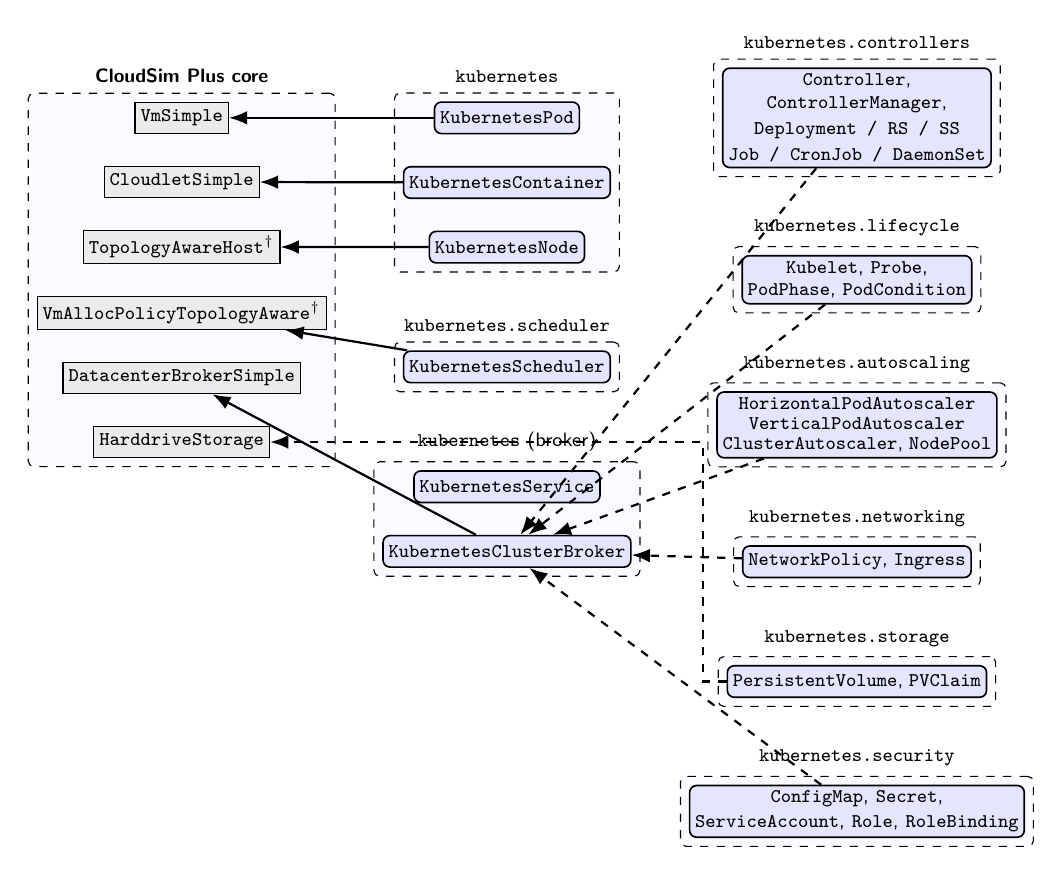
\begin{tikzpicture}[
            font=\scriptsize\sffamily,
            node distance=4mm and 5mm,
        % Existing CloudSim Plus core: sharp rectangle, light fill — B&W safe via shape.
            csp/.style={draw, rectangle, fill=black!8,
            minimum height=4mm, inner sep=2pt},
        % New K8s classes: rounded corners, light fill — distinguishable by shape under B&W.
            k8s/.style={draw, rounded corners=2.5pt, fill=blue!10, line width=0.6pt,
            minimum height=4mm, inner sep=2pt},
            pkg/.style={draw, dashed, rounded corners=2pt,
            inner sep=3pt, fill=blue!2},
            inh/.style={-Latex, thick},
            cmp/.style={-Latex, dashed, thick}
        ]
% --- Existing CSP layer (left) ---
            \node[csp] (vm)   {\texttt{VmSimple}};
            \node[csp,below=of vm] (clt) {\texttt{CloudletSimple}};
            \node[csp,below=of clt] (host) {\texttt{TopologyAwareHost}$^\dagger$};
            \node[csp,below=of host] (alloc) {\texttt{VmAllocPolicyTopologyAware}$^\dagger$};
            \node[csp,below=of alloc] (brk) {\texttt{DatacenterBrokerSimple}};
            \node[csp,below=of brk] (hdd) {\texttt{HarddriveStorage}};

% --- kubernetes (core entities) ---
            \node[k8s, right=26mm of vm] (pod) {\texttt{KubernetesPod}};
            \node[k8s, below=of pod] (ctr) {\texttt{KubernetesContainer}};
            \node[k8s, below=of ctr] (node) {\texttt{KubernetesNode}};

% --- scheduler ---
            \node[k8s, below=11mm of node] (sched) {\texttt{KubernetesScheduler}};

% --- broker / services ---
            \node[k8s, below=11mm of sched] (kservice) {\texttt{KubernetesService}};
            \node[k8s, below=of kservice] (kbroker) {\texttt{KubernetesClusterBroker}};

% --- right column: controllers / lifecycle / autoscaling / net / storage / sec ---
            \node[k8s, right=18mm of pod] (ctrls) {\shortstack{\texttt{Controller},\\\texttt{ControllerManager},\\\texttt{Deployment / RS / SS}\\\texttt{Job / CronJob / DaemonSet}}};

            \node[k8s, below=11mm of ctrls] (life) {\shortstack{\texttt{Kubelet}, \texttt{Probe},\\\texttt{PodPhase}, \texttt{PodCondition}}};

            \node[k8s, below=11mm of life] (auto) {\shortstack{\texttt{HorizontalPodAutoscaler}\\\texttt{VerticalPodAutoscaler}\\\texttt{ClusterAutoscaler},\;\texttt{NodePool}}};

            \node[k8s, below=11mm of auto] (net) {\texttt{NetworkPolicy},\;\texttt{Ingress}};

            \node[k8s, below=11mm of net] (stor) {\texttt{PersistentVolume},\;\texttt{PVClaim}};

            \node[k8s, below=11mm of stor] (sec) {\shortstack{\texttt{ConfigMap}, \texttt{Secret},\\\texttt{ServiceAccount}, \texttt{Role}, \texttt{RoleBinding}}};

% --- inheritance arrows (existing -> new) ---
            \draw[inh] (pod)   -- (vm);
            \draw[inh] (ctr)   -- (clt);
            \draw[inh] (node)  -- (host);
            \draw[inh] (sched) -- (alloc);
            \draw[inh] (kbroker)  -- (brk);

% --- composition arrows ---
            \draw[cmp] (ctrls) -- (kbroker);
            \draw[cmp] (life)  -- (kbroker);
            \draw[cmp] (auto)  -- (kbroker);
            \draw[cmp] (net)   -- (kbroker);
            \draw[cmp] (stor.west) -- ++(-3mm,0) |- (hdd.east);
            \draw[cmp] (sec)   -- (kbroker);

% --- package framing boxes: drawn on the background layer so their fill
% never paints over the entity nodes above, regardless of source order ---
            \begin{pgfonlayer}{background}
            \node[fit=(vm)(clt)(host)(alloc)(brk)(hdd), pkg, label=above:{\textbf{CloudSim Plus core}}] (cspbox) {};
            \node[fit=(pod)(ctr)(node), pkg, label=above:{\texttt{kubernetes}}] (k8score) {};
            \node[fit=(sched), pkg, label=above:{\texttt{kubernetes.scheduler}}] (kschedbox) {};
            \node[fit=(kservice)(kbroker), pkg, label=above:{\texttt{kubernetes} (broker)}] (kbrokbox) {};
            \node[fit=(ctrls), pkg, label=above:{\texttt{kubernetes.controllers}}] (ctrlsbox) {};
            \node[fit=(life), pkg, label=above:{\texttt{kubernetes.lifecycle}}] (lifebox) {};
            \node[fit=(auto), pkg, label=above:{\texttt{kubernetes.autoscaling}}] (autobox) {};
            \node[fit=(net), pkg, label=above:{\texttt{kubernetes.networking}}] (netbox) {};
            \node[fit=(stor), pkg, label=above:{\texttt{kubernetes.storage}}] (storbox) {};
            \node[fit=(sec), pkg, label=above:{\texttt{kubernetes.security}}] (secbox) {};
            \end{pgfonlayer}
        \end{tikzpicture}
        \caption{\ckm class hierarchy and package organisation.}
        \label{fig:arch}
    \end{figure*}

%%============================================================
    \section{Scheduling Algorithm}\label{sec:scheduling}
%%============================================================

    \subsection{Overview}

    The Kubernetes scheduler assigns each unbound pod to a node through a
    two-phase process: a \emph{filter} phase eliminates infeasible nodes,
    followed by a \emph{score} phase that ranks feasible candidates.
    \ckm models this with the scheduler, which extends the allocation
    policy and overrides its filter and scoring methods. Non-Kubernetes
    \texttt{Vm}/\texttt{Host} pairs fall through to the parent policy
    unchanged, making the scheduler transparent to mixed-workload
    simulations.

    \subsection{Filter Phase}

    The filter phase eliminates nodes that violate hard constraints:
    resource capacity, nodeSelector labels, required NodeAffinity,
    taint/toleration enforcement, and required pod affinity rules.
    Topology buckets for pod affinity are determined by a TopologyKey:
    HOSTNAME (same physical node), ZONE (same availability zone), or
    REGION (same geographic region), reusing the existing CloudSim Plus
    topology infrastructure.

    \subsection{Tie-Breaking Strategies}\label{sec:tie-break}

    When multiple feasible nodes receive the same score, the upstream
    kube-scheduler delegates to a \texttt{SchedulingProfile} extension
    that, in production, performs a seeded randomisation for fairness.
    The tie-break strategy is configurable; the default is lexicographic
    order, which is fully deterministic across JVMs and ensures
    reproducible RQ1 results. A seeded-random variant is available for
    studies that require stochastic tie-breaking to match the production
    scheduler's behaviour; a 5-run sensitivity sweep is reported in
    Section~\ref{sec:external-validation} so that the deterministic
    headline number can be compared against the stochastic distribution.
    Cross-tool agreement against
    \texttt{kube-scheduler-simulator}~\cite{KubeSchSim2025} --- which runs
    the production \texttt{kube-scheduler} binary against a synthetic
    cluster state --- is reported in Section~\ref{sec:external-validation}
    as the primary fidelity comparator: both the headline (deterministic
    tie-break) and the 5-run sensitivity sweep are computed against
    \texttt{kube-scheduler-simulator}'s placement decisions on the
    identical RQ1 scenario set. An auxiliary method exposes the full
    tied-minimum-score set, supporting score-set agreement metrics where
    exact-winner agreement is too sensitive to tie-break choice; this is
    the score-set coverage figure reported in
    Section~\ref{sec:external-validation} alongside the headline winner
    agreement.

%%============================================================
    \section{Control Plane Simulation}\label{sec:controlplane}
%%============================================================

    The control plane in \ckm reconstructs the four
    behaviours that determine pod lifecycle in a real Kubernetes
    cluster: periodic reconciliation of declared vs.\ observed state,
    workload-controller-driven pod creation and rollout, kubelet-side
    pre-flight admission and probing, and label-selector-based service
    discovery. The following four subsections describe each in turn.

    \subsection{Tick-Driven Reconciliation}

    Kubernetes controllers operate as continuous reconciliation loops:
    each iteration compares the \emph{observed state} of the cluster to
    the \emph{desired state} declared in a resource specification and
    takes corrective action. \ckm models this through a periodic tick
    callback invoked by the cluster broker every configurable simulated
    interval (default 1.0\,s). Each controller, the Kubelet, and the
    autoscalers implement the tick interface, enabling independent
    reconciliation cadences if required.

    The controller manager routes pod lifecycle events (creation,
    deletion, failure) to the owning controller via owner-reference
    labels stamped on each pod at creation time. This decouples
    controller implementations from the broker and supports multiple
    simultaneous controllers without explicit registration.

    \subsection{Workload Controllers}

    Table~\ref{tab:controllers} summarises the six workload controller
    types implemented in \ckm.

    \begin{table*}[!t]
        \centering
        \caption{Workload controller types and their simulation
        semantics.\label{tab:controllers}}
        \footnotesize
        \begin{tabular*}{\textwidth}{@{\extracolsep{\fill}}p{0.21\textwidth}p{0.40\textwidth}p{0.30\textwidth}@{}}
\toprule
\textbf{Controller} & \textbf{Reconciliation Semantics} & \textbf{Key Parameters} \\
\midrule
\texttt{ReplicaSetController} & Maintain desired replica count; create/delete pods & \texttt{desiredReplicas}, \texttt{podTemplate} \\
\texttt{DeploymentController} & Rolling transition between old/new ReplicaSet & \texttt{updateStrategy} (maxSurge, maxUnavailable) \\
\texttt{StatefulSetController} & Ordinal-stable naming (\texttt{pod-0}, \texttt{pod-1}, \ldots) & \texttt{desiredReplicas}, ordinal index \\
\texttt{JobController} & Spawn pods up to parallelism; count completions & \texttt{completions}, \texttt{parallelism}, \texttt{backoffLimit} \\
\texttt{CronJobController} & Trigger \texttt{JobController} on cron expression or interval & \texttt{cronExpression} (UNIX/Quartz/etc.) or \texttt{schedule} \\
\texttt{DaemonSetController} & Ensure exactly one pod per schedulable node; opt-in rolling update & node set, pod template, \texttt{updateStrategy} \\
\bottomrule
        \end{tabular*}
    \end{table*}

    Six workload controller types are implemented under a tick-driven
    reconciliation loop (Table~\ref{tab:controllers}). Each controller
    reconciles observed versus desired state every configurable tick
    interval; the Kubelet sequences init containers and enforces
    liveness, readiness, and startup health probes before marking a pod
    Running.

    \subsection{Kubelet and Pod Lifecycle}

    The \texttt{Kubelet} manages the container lifecycle for all pods
    hosted on a broker's nodes. Figure~\ref{fig:lifecycle} presents the
    pod state machine: a pod advances \texttt{Submitted}\,$\to$\,
    \texttt{PENDING}\,$\to$\,init containers\,$\to$\,\texttt{RUNNING}\,$\to$\,
    \texttt{SUCCEEDED} along the solid normal-progression arrows. The dashed
    red arrows are the failure/restart transitions: an init-container
    failure, or a main-container failure that reaches the pod's
    \texttt{backoffLimit}, drives the pod to the terminal \texttt{FAILED}
    state (grey boxes are terminal). \texttt{READY} (dotted, above
    \texttt{RUNNING}) is a compound condition set only once all main
    containers pass their readiness probes; until it holds, the pod is
    gated from receiving traffic through \texttt{KubernetesService}. These
    transitions are triggered by scheduler decisions, container events,
    and probe outcomes.

    \begin{figure*}[!t]
        \centering
        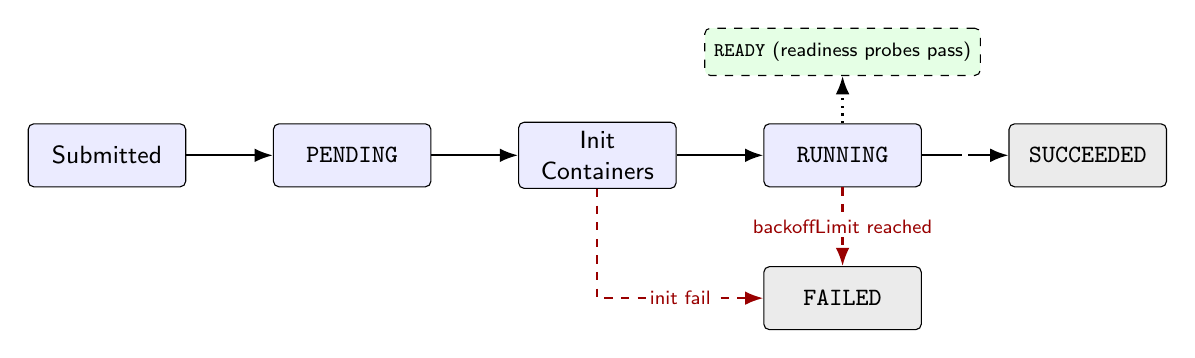
\begin{tikzpicture}[
            font=\small\sffamily,
            node distance=10mm and 11mm,
            state/.style={draw, rounded corners=2pt, minimum height=8mm,
            minimum width=20mm, fill=blue!8, align=center},
            term/.style={draw, rounded corners=2pt, minimum height=8mm,
            minimum width=20mm, fill=black!8, align=center},
            cond/.style={draw, dashed, rounded corners=2pt, minimum height=6mm,
            minimum width=20mm, fill=green!10, align=center,
            font=\scriptsize\sffamily},
            norm/.style={-Latex, thick},
            fail/.style={-Latex, thick, dashed, red!60!black},
            edgelbl/.style={font=\scriptsize\sffamily, fill=white, inner sep=1pt}
        ]
% --- top row: linear lifecycle ---
            \node[state]                                    (sub)  {Submitted};
            \node[state, right=of sub]                      (pen)  {\texttt{PENDING}};
            \node[state, right=of pen]                      (init) {Init\\Containers};
            \node[state, right=of init]                     (run)  {\texttt{RUNNING}};
            \node[term,  right=of run]                      (suc)  {\texttt{SUCCEEDED}};

% --- terminal failure node, centered below RUNNING for short, clean arrows ---
            \node[term,  below=10mm of run]                 (fail) {\texttt{FAILED}};

% --- READY condition, attached to RUNNING ---
            \node[cond, above=6mm of run]                   (rdy)  {\texttt{READY} (readiness probes pass)};

% normal flow
            \draw[norm] (sub)  -- (pen);
            \draw[norm] (pen)  -- (init);
            \draw[norm] (init) -- (run);
            \draw[norm] (run)  -- node[edgelbl]{}   (suc);

% READY condition gating from RUNNING
            \draw[norm, dotted] (run) -- (rdy);

% failure transitions: short straight verticals
            \draw[fail] (init) |- node[edgelbl, pos=0.75]{init fail} (fail);
            \draw[fail] (run)  -- node[edgelbl]{backof{}fLimit reached}                       (fail);
        \end{tikzpicture}
        \caption{Pod lifecycle state machine governed by the Kubelet.}
        \label{fig:lifecycle}
    \end{figure*}

    Upon pod placement the Kubelet sequences init containers before
    starting main containers. Each init container is submitted as a
    cloudlet and monitored to completion; only after all init containers
    succeed are main containers started concurrently. Liveness and
    readiness probes are evaluated on each Kubelet tick: a failed
    liveness probe triggers a container restart (subject to the pod's
    restart policy); a failed readiness probe gates the pod from
    receiving traffic through \texttt{KubernetesService}.

    \subsection{Service Discovery}

    \texttt{KubernetesService} resolves its backing endpoints
    dynamically on every \texttt{selectVm()} invocation: it filters the
    full pod list to those that are created, in the correct namespace, and
    whose labels match the service's \texttt{LabelSelector}, and
    additionally requires \texttt{PodCondition.READY} (unless no pods are
    ready yet, in which case pre-ready pods are included to avoid
    starvation). Round-robin selection among backing pods is implemented
    with a wraparound index.

%%============================================================
    \section{Autoscaling}\label{sec:autoscaling}
%%============================================================

    \subsection{Horizontal Pod Autoscaler}

    The \texttt{HorizontalPodAutoscaler} (HPA) adjusts the replica count
    of a target workload controller based on average CPU utilisation
    across managed pods, implementing the standard Kubernetes HPA control law~\cite{KubernetesDocs}:

    \begin{equation}\label{eq:hpa}
        d^* = \left\lceil d_{\mathrm{curr}} \cdot
                  \frac{\bar{u}_{\mathrm{cpu}}}{\tau_{\mathrm{cpu}}} \right\rceil
    \end{equation}

    where $d_{\mathrm{curr}}$ is the current replica count,
    $\bar{u}_{\mathrm{cpu}}$ is the mean CPU utilisation across the set of
    \emph{Ready} pods (matching real Kubernetes, which excludes pods
    scheduled but not yet passing their readiness probe from the metric
    sample), $\tau_{\mathrm{cpu}} \in (0,1]$ is the target utilisation
    threshold, and $d^*$ is clamped to $[d_{\min}, d_{\max}]$. Scaling
    decisions are gated by two complementary mechanisms that mirror the
    Kubernetes 1.18+ HPA. First, a \emph{tolerance window} (default
    $\pm10\,\%$, controlled by \texttt{tolerance}) suppresses
    recommendations while $|\bar{u}_{\mathrm{cpu}} -
    \tau_{\mathrm{cpu}}|/\tau_{\mathrm{cpu}} < \mathrm{tolerance}$,
    eliminating the flutter that a tolerance-free controller would
    otherwise produce. Second, asymmetric stabilisation
    windows---\texttt{cooldownScaleUpSeconds} (default $0$\,s) and
    \texttt{cooldownScaleDownSeconds} (default $300$\,s)---throttle
    scale-up and scale-down separately, matching K8s'
    \texttt{behavior.scaleUp} / \texttt{scaleDown.stabilizationWindowSeconds}
    defaults. A legacy single-cooldown setter
    (\texttt{cooldownSeconds}, default 60\,s) sets both buckets identically
    to preserve backward compatibility (Algorithm~\ref{alg:hpa}). Container
    CPU utilisation is sourced from
    \texttt{KubernetesContainer.getCpuPercentUtilization()}, which
    delegates to the cloudlet's utilisation model---enabling realistic
    HPA dynamics when containers are wired to \texttt{UtilizationModelDynamic}
    or \texttt{UtilizationModelPlanetLab} traces rather than
    constant-100\% models. Equation~\eqref{eq:hpa} is shown for CPU
    utilisation, which is the only metric the framework currently samples;
    memory, request-rate, and external-metrics HPAs (upstream's
    \texttt{type: Resource/Pods/Object/External}) are listed in
    Section~\ref{sec:simplifications} as deferred extension points reusing
    the same formula on a different signal.

    \begin{algorithm}[t]
\caption{HPA Reconciliation Loop}\label{alg:hpa}
\begin{algorithmic}[1]
    \Procedure{Tick}{$t$}
        \State $P \leftarrow \{\,p \in \mathrm{controller.managedPods()} : p.\mathrm{isReady}()\,\}$
            \Comment{Ready pods only}
        \If{$P = \emptyset$} \State \textbf{return} \EndIf
        \State $\bar{u} \leftarrow \mathrm{mean}\{\,p.\mathrm{cpuUtil}() : p \in P\,\}$
        \If{$\bar{u} \le 0 \;\lor\; |\bar{u} - \tau|/\tau < \mathrm{tol}$} \State \textbf{return}
            \Comment{Tolerance band} \EndIf
        \State $d^* \leftarrow \mathrm{clamp}\!\left(\left\lceil d_{\mathrm{curr}} \cdot
                                                         \bar{u}/\tau \right\rceil,\;[d_{\min}, d_{\max}]\right)$
        \If{$d^* = d_{\mathrm{curr}}$} \State \textbf{return} \EndIf
        \State $\mathrm{cd} \leftarrow (d^* > d_{\mathrm{curr}})\;?\;
            \mathrm{cd}_{\uparrow}\;:\;\mathrm{cd}_{\downarrow}$
            \Comment{Asymmetric cooldown}
        \If{$t - t_{\mathrm{scale}} < \mathrm{cd}$} \State \textbf{return} \EndIf
        \State controller.setDesiredReplicas$(d^*)$;\quad
            $t_{\mathrm{scale}} \leftarrow t$
    \EndProcedure
\end{algorithmic}
    \end{algorithm}

    \subsection{Cluster Autoscaler}

    The \texttt{ClusterAutoscaler} operates at the infrastructure layer,
    provisioning or decommissioning nodes from a \texttt{NodePool}
    (bounded by \texttt{min}/\texttt{max} node counts) in response to
    scheduling pressure (Algorithm~\ref{alg:ca}).

    \textbf{Scale-up} is triggered when unschedulable pods exist and the
    pool has not reached its maximum: a new node is instantiated from the
    pool's template supplier, added to the datacenter via
    \texttt{Datacenter.addHost()}, and unschedulable pods are cleared and
    resubmitted for placement.

    \textbf{Scale-down} is triggered when a node has been idle (no
    running pods) for at least \texttt{scaleDownAfterSeconds} (default
    600\,s) and removal would not violate the pool's minimum. Both actions
    are subject to a shared cooldown (default 30\,s).

    \begin{algorithm}[t]
\caption{Cluster Autoscaler Reconciliation}\label{alg:ca}
\begin{algorithmic}[1]
    \Procedure{Tick}{$t$}
        \If{$t - t_{\mathrm{act}} < \mathrm{cooldown}$} \State \textbf{return} \EndIf
        \State $P_u \leftarrow \{p : p.\mathrm{isUnschedulable} \wedge \neg p.\mathrm{isCreated}\}$
        \If{$P_u \ne \emptyset \wedge \mathrm{prov} < \mathrm{pool.max}$}
            \State $n \leftarrow \mathrm{pool.template.get()}$;\quad add $n$ to datacenter
            \State $\mathrm{prov} \mathrel{+}= 1$;\quad $t_{\mathrm{act}} \leftarrow t$
            \State clear unschedulable flags; resubmit $P_u$;\quad\textbf{return}
        \EndIf
        \ForAll{$n \in \mathrm{pool}$ with $\mathrm{pods}(n) = \emptyset$}
            \If{$t - \mathrm{idleSince}(n) \ge \mathrm{scaleDownAfter}$}
                \If{$\mathrm{pool.size} - 1 \ge \mathrm{pool.min}$}
                    \State decommission $n$;\quad $\mathrm{prov} \mathrel{-}= 1$;\quad
                    $t_{\mathrm{act}} \leftarrow t$
                \EndIf
            \EndIf
        \EndFor
    \EndProcedure
\end{algorithmic}
    \end{algorithm}

    \subsection{Vertical Pod Autoscaler}\label{sec:vpa}

    The \texttt{VerticalPodAutoscaler} samples per-container CPU and memory
    utilisation across a target \texttt{ReplicaSetController}'s managed
    pods on every tick and exposes sizing recommendations via
    \texttt{getRecommendedMilliCpu()} / \texttt{getRecommendedMemMiB()}.
    Three operating modes mirror the upstream Kubernetes VPA
    \texttt{updatePolicy.updateMode}: \textbf{Off} and \textbf{Initial}
    surface recommendations without automatic mutation (default);
    \textbf{Auto} applies recommendations \emph{in-place} by patching each
    container's \texttt{effectiveLimits} field, leaving the pod object
    intact, mirroring the K8s 1.27+ \texttt{InPlacePodVerticalScaling}
    behaviour for CPU (compressible; no restart) and applying memory limit
    updates without a restart as a documented simplification
    (Section~\ref{sec:simplifications}). Auto-recreate via pod eviction
    remains opt-in through \texttt{setEvictOnRecommendation(true)}.
    Recommendations are gated by the same tolerance and cooldown machinery
    used by the HPA, mirroring the upstream VPA recommender's deadband and
    rate-limiter.

    \subsection{Two-Tier Autoscaler Interaction}

    The two autoscalers interact synergistically: HPA scale-out may
    produce unschedulable pods when no node has sufficient capacity,
    which in turn triggers Cluster Autoscaler scale-up. Conversely, HPA
    scale-in drains nodes to zero pods, eventually triggering
    Cluster Autoscaler scale-down. This interaction reproduces the
    two-tier Kubernetes autoscaling architecture and enables study of
    oscillation, contention, and tuning strategies that are active
    research topics in the Kubernetes scheduling literature~\cite{Li2023}.

    \subsection{M/M/c Calibration Recipe}\label{sec:mmc-calibration}

    The trace-comparison results of Section~\ref{sec:online-boutique}
    rest on per-service \texttt{M/M/c} queueing draws performed by the
    \texttt{kubernetes.networking.queueing} sub-package. We specify the
    parameterisation in full so that the reported $\log_{10}$ ratios are
    reproducible.

    \textbf{Arrival rate} ($\lambda$). The real-side offered rate is
    recorded at the HTTP frontend (the loadgenerator's per-endpoint
    counters in \texttt{real-latency.csv}); it is not broken down per
    backend gRPC operation, so the per-operation queue draws cannot read a
    measured $\lambda_{s,op}$ directly. Instead, for each elastic service
    the queue is driven at the analytic rate $\lambda = \rho \cdot c \cdot
    \mu$ implied by its calibrated per-pod utilisation $\rho$ and
    steady-state replica count $c$ --- i.e.\ $\lambda$ is the drive rate
    that reproduces the calibrated load on the modelled queue, not an
    independently measured arrival count. Within a window we assume a
    homogeneous Poisson process; bursts within the window are not
    separately modelled. This is the standard M/M/c arrival assumption, but we flag
    it as an approximation rather than an exact match: a closed-loop,
    think-time-free Locust workload is a \emph{closed} system (a bounded
    user population, each user issuing its next request only after the
    previous response returns), not an open Poisson stream, so the true
    arrival process is not memoryless and self-throttles as the system
    fills. We return to this in Section~\ref{sec:threats}.

    \textbf{Service rate} ($\mu$). $\mu_{s,op}$ is calibrated once per
    service from the upstream Boutique microbenchmarks shipped with
    \texttt{microservices-demo} and stored in a json file.
    For \texttt{recommendationservice/ListRecommendations} the calibrated
    per-replica value is $\mu = 410$ req/s (a mean service time
    $\mu^{-1} \approx 2.4\,$ms); each backing pod's queue is modelled with
    this rate per server.

    \textbf{Number of servers} ($c$). $c$ is the \emph{steady-state replica
    count} of the backing Deployment under the HPA --- the post-scale-up
    plateau, not the initial replica count. The simulator derives this
    plateau deterministically from the calibrated load and the HPA's
    $[\textrm{minReplicas}, \textrm{maxReplicas}]$ bounds, and it equals
    the live count the latency-CSV path re-reads from the Deployment at
    finalisation, so the trace-side and CSV-side latency models use the
    same $c$. Sizing the queue at the initial $c{=}1$ instead would
    saturate every elastic queue and silently under-estimate throughput.

    \textbf{Granularity}. One M/M/c queue model instance per service
    (not per operation), keyed by service name. Operations on the same
    service share the model; the comparator distinguishes them by
    operation name in the resulting Jaeger spans.

    \textbf{Worked example.} For \texttt{ListRecommendations} at
    200 Locust users on the Online Boutique substrate, the trace
    generator's M/M/c queue is provisioned with $\mu = 410$ req/s per
    replica and $c = 3$ servers --- the HPA steady-state replica count of
    \texttt{recommendationservice} on this load (the
    \texttt{maxReplicas}-capped plateau confirmed in
    Sections~\ref{sec:threats} and~\ref{sec:online-boutique}, where each
    pod runs at $\approx\!85\%$ CPU against a target $\tau = 0.70$). The
    per-pod load is held at $\rho = 0.85$, so the queue is driven at
    $\lambda = \rho \cdot c \cdot \mu = 1{,}046$ req/s (an analytic drive
    rate computed from the calibrated load, not a measured offered rate;
    see the arrival-rate note above), giving per-replica utilisation
    $\rho = \lambda / (c \cdot \mu) = 0.850$: inside the M/M/c stability
    bound but firmly in the queueing regime, so the $p95$ is dominated by
    Erlang-C wait time rather than raw service time. The wait-time draw
    plus the exponential service-time draw yields $p95_\textrm{sim} =
    17{,}875\,\mu$s versus $p95_\textrm{real} = 46{,}383\,\mu$s ---
    the $\log_{10} = -0.41$ headline match
    (Table~\ref{tab:boutique-results}); the simulator is $\approx\!2.6\times$
    faster than the real handler, the closest of the eight operations but
    still a mild under-prediction. The tuple above is emitted verbatim by
    the example (\texttt{WORKED-EXAMPLE} log line) so the calibration is
    reproducible. Operations whose real handler returns below the M/M/c
    service-time floor ($\mu^{-1} \approx 2.4\,\textrm{ms}$ at
    $\rho \to 0$) cannot be matched by this model regardless of
    calibration; these are listed in the residual simplifications
    (Section~\ref{sec:simplifications}).

    \subsection{Modelled Simplifications}\label{sec:simplifications}

    The framework provides event-level fidelity within the scope of the
    simplifications enumerated below, not bitwise equivalence with the
    upstream control plane: a discrete-event simulator of an
    orchestration system as large as Kubernetes must trade off
    control-flow faithfulness against engineering tractability. Every
    deliberate simplification is enumerated in
    Table~\ref{tab:simplifications} --- each row pairing a modelled aspect
    (e.g.\ Job pod completion, CronJob scheduling) with its simulation
    semantics or its documented divergence from upstream --- so that
    reviewers, downstream researchers, and benchmark authors can reason
    precisely about the bounds of validity. The \textbf{ID} column reuses
    the M-series and S-series keys of Table~\ref{tab:simpl-tests}, which
    maps each identifier to its pinning regression test; ``---'' marks
    aspects that are modelled but do not carry a short-form contract ID.
    The closing validation-gate clause (S-GATE) is stated in the text
    below the table.

    \begin{table*}[!t]
        \centering
        \caption{Modelled simplifications of \ckm.\label{tab:simplifications}}
        \footnotesize
        \setlength{\tabcolsep}{4pt}
        \begin{tabular*}{\textwidth}{@{\extracolsep{\fill}}@{}l p{0.225\textwidth} p{0.58\textwidth}@{}}
\toprule
\textbf{ID} & \textbf{Aspect} & \textbf{Modelled semantics / documented divergence from upstream} \\
\midrule
M4              & Job pod completion            & Mirrors real K8s Job semantics, including \texttt{backoffLimit}-driven retries. \\
\addlinespace
M8              & CronJob scheduling            & Accepts either a fixed simulated-second period or a full cron expression (UNIX, Quartz, Spring, cron4j flavours via the \emph{cron-utils} library); the full Kubernetes API surface (\texttt{concurrencyPolicy}, \texttt{startingDeadlineSeconds}, per-firing replacement) is honoured. \\
\addlinespace
M3              & Pod memory aggregation        & Pod-level memory uses $\sum_c \mathrm{limits}(c).\mathrm{memMiB}$; the container enforces \texttt{limits}~$\geq$~\texttt{requests} at construction time. \\
\addlinespace
M2/N6           & Resource parsers              & CPU rounds via $\mathrm{round}(\text{double} \cdot 1000)$ to the nearest millicore, matching the K8s \texttt{Quantity} parser. Sub-MiB memory inputs floor to a 1\,MiB minimum. \\
\addlinespace
M5/M6           & DaemonSet on YAML clusters    & Every node carries a \texttt{kubernetes.io/hostname} label by default, so DaemonSet pinning works regardless of cluster build path. \\
\addlinespace
---             & Image pull latency            & Pods become \texttt{Running} immediately on placement, modulo kubelet pre-flight on declared ConfigMaps, Secrets, ServiceAccounts, and bound PVCs. \\
\addlinespace
---             & Vertical Pod Autoscaler       & Supports the three K8s VPA modes (\texttt{OFF}, \texttt{INITIAL}, \texttt{AUTO}). \texttt{AUTO} applies in-place CPU resize (K8s 1.27+ \texttt{InPlacePodVerticalScaling}); QoS-class reclassification side-effects on memory updates are not modelled. \\
\addlinespace
---             & NetworkPolicy                 & Enforcement is ingress-only at namespace + pod-selector level. Per-source pod-to-pod policies, port ranges, and egress rules are not modelled. \\
\addlinespace
---             & RBAC enforcement              & \texttt{Role}/\texttt{RoleBinding} carry metadata only; verb/resource authorisation is not simulated. The kubelet pre-flight refuses pods whose declared \texttt{ServiceAccount} is not registered. \\
\addlinespace
---             & PersistentVolume model        & PVC binding is first-fit at registration time, matched on capacity, storage class, and label selector. Reclaim policies, dynamic provisioning, and in-tree volume plugins are not modelled. \\
\addlinespace
S-PDB           & PodDisruptionBudget           & Scale-down does not consult a PDB equivalent. \\
\addlinespace
S-CA-COOLDOWN   & Cluster Autoscaler cooldowns  & A single shared cooldown gates both scale-up and scale-down; upstream's three separate delay timers are not modelled. \\
\addlinespace
S-TSC           & TopologySpreadConstraints     & First-class \texttt{topologySpreadConstraints} objects are not implemented; equivalent spread is achievable through \texttt{COST\_OPTIMIZED} placement side-effects and pod anti-affinity. \\
\addlinespace
S-SIDECAR       & Sidecar containers            & The K8s 1.28 native sidecar lifecycle is not distinguished from regular main containers. \\
\addlinespace
S-POD-RES       & Pod-level resources           & Pod-level CPU/memory budgets introduced in Kubernetes 1.32 are not modelled. \\
\addlinespace
S-ENDPOINTSLICE & Endpoint model                & Services maintain a single round-robin endpoint list under the legacy Endpoints model; EndpointSlice sharding is not modelled. \\
\addlinespace
S-TGS           & Graceful shutdown             & \texttt{terminationGracePeriodSeconds}, PreStop hooks, and the \texttt{SIGTERM}~$\to$~\texttt{SIGKILL} sequence are not modelled. \\
\addlinespace
S-RUNTIME       & Pod overhead / RuntimeClass   & No \texttt{RuntimeClass} object; \texttt{spec.overhead} budget for gVisor/Kata/Firecracker runtimes is not accounted for. \\
\addlinespace
S-VOL           & Ephemeral and CSI volumes     & Only static \texttt{PersistentVolume}~+~\texttt{PersistentVolumeClaim} binding is implemented. Ephemeral inline volumes, CSI drivers, dynamic provisioning, and online volume expansion are not modelled. \\
\addlinespace
S-HPA-METRICS   & Custom-metrics HPA            & The HPA samples CPU utilisation only; custom, object, and external metrics are not yet implemented. \\
\addlinespace
S-PULL          & Image pull policy             & \texttt{imagePullPolicy}, image-pull latency, image-pull Secret authentication, and registry-rate-limit back-off are not modelled. \\
\addlinespace
S-KUBEPROXY     & Service load-balancing model  & Round-robin draw over Ready pods. kube-proxy iptables vs.\ IPVS choice, session-affinity, \texttt{externalTrafficPolicy}, and \texttt{internalTrafficPolicy} are not modelled. \\
\addlinespace
S-GATEWAY       & Gateway API                   & Only the legacy \texttt{Ingress} resource is modelled; \texttt{Gateway}, \texttt{HTTPRoute}, \texttt{GRPCRoute}, and \texttt{TCPRoute} are out of scope. \\
\bottomrule
        \end{tabular*}
    \end{table*}

    \noindent\textbf{Validation gate (S-GATE).}~The entries of
    Table~\ref{tab:simplifications} are the principal documented
    divergences from upstream Kubernetes; every one is exercised by at
    least one regression test, as listed in Table~\ref{tab:simpl-tests}.
    Any \ckm behaviour outside this list that diverges from upstream is
    treated as a bug, fixed, and accompanied by a new test.

    \noindent\textbf{Defect history.}~A senior-engineering review and
    the subsequent saturation-regime trace work together identified
    eight defects spanning four categories: filter-phase scoring math
    (\texttt{TaintTolerationPriority}), controller-loop classification
    (Pending pods marked ``lost'' by the ReplicaSet reconciliation),
    trace-generator queue construction (elastic-callee spans dropped
    when the queue was built from \texttt{svc.replicas} under
    effective load $>1$), and topology-aware placement edge cases.
    All eight are now pinned by regression tests in
    Table~\ref{tab:simpl-tests} or the broader 214-test suite
    (Section~\ref{sec:external-validation}). Every identifier from
    Section~\ref{sec:simplifications} appears in that table, paired with
    the regression test class that pins it; \emph{absent} indicates a
    gap-by-design that the contract surfaces, and closing each absent
    entry is a unit of follow-up work (Section~\ref{sec:conclusions}).

    \begin{table*}[!t]
        \centering
        \caption{Simplification-to-test mapping.\label{tab:simpl-tests}}
        \footnotesize
        \setlength{\tabcolsep}{6pt}
        \begin{tabular*}{\textwidth}{@{\extracolsep{\fill}}lll@{}}
\toprule
\textbf{ID} & \textbf{Simplification} & \textbf{Pinning test} \\
\midrule
M2/N6           & Resource parsers (CPU/memory)         & \texttt{ResourcesParsingModeTest}, \texttt{ResourcesTest} \\
M3              & Pod memory aggregation                & \texttt{KubernetesPodTest} \\
M4              & Job pod completion + backoff          & \texttt{JobControllerBackoffTest} \\
M5/M6           & DaemonSet hostname labelling          & \texttt{DaemonSetRollingUpdateTest} \\
M8              & CronJob expression / concurrency      & \texttt{CronJobExpressionTest} \\
---             & Image pull pre-flight                 & \texttt{KubeletPreflightTest} \\
---             & VPA modes incl.\ in-place Auto        & \texttt{VerticalPodAutoscalerTest} \\
---             & NetworkPolicy ingress                 & \texttt{NetworkPolicyTest} \\
---             & RBAC metadata-only enforcement        & \texttt{SecurityModelTest}, \texttt{KubeletPreflightTest} \\
---             & PV / PVC first-fit binding            & \texttt{PersistentVolumeTest} \\
S-PDB           & PodDisruptionBudget                   & absent --- gap-by-design \\
S-CA-COOLDOWN   & Single shared CA cooldown             & \texttt{NodePoolTest}, \texttt{KubernetesAutoscalingTest} \\
S-TSC           & \texttt{topologySpreadConstraints}    & absent --- gap-by-design \\
S-SIDECAR       & K8s 1.28 native sidecar lifecycle     & absent --- gap-by-design \\
S-POD-RES       & Pod-level CPU/memory budgets (1.32)   & absent --- gap-by-design \\
S-ENDPOINTSLICE & Endpoints round-robin (legacy)        & \texttt{KubernetesServiceTest} \\
S-TGS           & \texttt{terminationGracePeriodSeconds}& absent --- gap-by-design \\
S-RUNTIME       & RuntimeClass / \texttt{spec.overhead} & absent --- gap-by-design \\
S-VOL           & Static PV+PVC only                    & \texttt{PersistentVolumeTest} \\
S-HPA-METRICS   & CPU-only HPA metrics                  & \texttt{HorizontalPodAutoscalerTest}, \texttt{HpaTrajectoryShapeTest} \\
S-PULL          & \texttt{imagePullPolicy} / back-off   & absent --- gap-by-design \\
S-KUBEPROXY     & Round-robin service LB                & \texttt{KubernetesServiceTest} \\
S-GATEWAY       & Legacy Ingress only                   & \texttt{IngressTest} \\
S-GATE          & Validation gate (suite-wide)          & \texttt{Kubernetes*Test} integration suites \\
\bottomrule
        \end{tabular*}
    \end{table*}

%%============================================================
    \section{Validation and Evaluation}\label{sec:validation}
%%============================================================

    \subsection{External Validation on a 4-Node k3s Cluster}\label{sec:external-validation}

    The extension ships with 214 unit and integration tests. The suite pins component
    contracts and every documented simplification of
    Section~\ref{sec:simplifications} via the mapping in
    Table~\ref{tab:simpl-tests}. We additionally report empirical
    agreement against a live Kubernetes cluster: an Oracle Cloud k3s
    cluster with one control plane and three worker nodes
    (k3s \texttt{v1.35.4+k3s1}, each node 1\,vCPU / 6\,GiB RAM).
    The cross-tool comparator is
    \texttt{kube-scheduler-simulator}~\cite{KubeSchSim2025}
    \texttt{v0.4.0}, run over a KWOK fake cluster under Docker Compose;
    the full evaluation toolchain is pinned at JDK~25.0.1, k3s
    \texttt{v1.35.4+k3s1}, Jaeger \texttt{all-in-one:1.57}, the
    OpenTelemetry Collector \texttt{contrib:0.103.0}, and Google Online
    Boutique (\texttt{microservices-demo}) at tag \texttt{v0.10.1}.
    Synthetic \texttt{topology.kubernetes.io/zone} and \texttt{rack}
    labels are applied to the three workers so that
    rack and zone affinity scenarios are exercised end-to-end on
    the existing substrate, and \texttt{kube-scheduler-simulator}
    serves as the primary cross-tool comparator for the broader
    RQ1 fidelity claim, as detailed in Section~\ref{sec:threats}.
    Cluster Autoscaler real-cluster validation remains in the simulator
    only because Oracle k3s ships no built-in Cluster Autoscaler; its
    scope boundary is also documented in Section~\ref{sec:threats}.

    The protocol is structured around five research
    questions~\cite{Pucher2015}.

    \textbf{RQ1: Scheduling Fidelity.} How closely does \ckm
    replicate the placement decisions of the production
    \texttt{kube-scheduler} on a fixed scenario set We generated 300
    deterministic pod-placement scenarios varying labels,
    \texttt{nodeSelector}, required \texttt{nodeAffinity}, and
    tolerations, then compared placements on \emph{two substrates}:
    (i)~the production \texttt{kube-scheduler} binary running under
    \texttt{kube-scheduler-simulator}~\cite{KubeSchSim2025} on the local
    machine --- the primary comparator, because it executes the exact
    upstream scheduler code and admits thousands of scenarios at zero
    hardware cost; and (ii)~the 3-worker real-cluster substrate, where
    the same workers have been re-labelled with synthetic
    \texttt{topology.kubernetes.io/zone}, \texttt{rack}, and
    \texttt{region} labels so that the
    scenarios actually exercise the topology-spread filter and score
    predicates that a uniform 3-worker substrate would otherwise leave
    unreached. The kss cluster is seeded to match the simulator's
    modelled state (the two background pods on \texttt{worker-1}/%
    \texttt{worker-2}) so both engines score an identical cluster. The
    simulator side runs with the default \texttt{lexical()} tie-break
    throughout; the 5-run sensitivity sweep re-runs the
    \texttt{kube-scheduler} side, whose per-run randomised tie-break is
    the only stochastic element.
    \emph{Targets}: $\geq 60\%$ strict winner-node agreement against
    \texttt{kube-scheduler-simulator}, rising to $\geq 80\%$ for the
    combined winner-or-score-set metric; the real-cluster substrate is
    reported separately as a secondary check, where combined agreement
    reaches $\geq 95\%$.

    \textbf{RQ2: HPA Behavioural Validity.} Does the Horizontal Pod
    Autoscaler reproduce the scaling trajectory of real Kubernetes under
    representative workloads? We deployed a CPU-bound web service on the
    real cluster driven by 1{,}000 concurrent Locust users, ran the
    equivalent scenario through the simulator, and computed pod-count
    NRMSD and steady-state replica error.
    \emph{Targets}: steady-state replica error $= 0$\,pods; pod-count
    NRMSD $< 0.20$ on the raw (un-aligned) trajectory and $< 0.15$ after
    phase-alignment, reported both ways.

    \textbf{RQ2b: VPA Recommendation Accuracy.} Does the simulator's VPA
    recommendation formula match the real Kubernetes VPA recommender at
    steady state? We deployed a CPU-burn workload on the real cluster
    with VPA recommender v1.6.0 in Off mode, sampled recommendations over
    7.5\,min, and compared against the simulator's formula.
    \emph{Target}: steady-state recommendation error $< 5\%$.

    \textbf{RQ3: Simulation Scalability.} How does simulation wall-clock
    time scale with node count and pod count? We ran synthetic cluster
    benchmarks sweeping $n \in \{10, 100, 1{,}000\}$ nodes at fixed
    $p = 100$ pods and $p \in \{100, 500, 1{,}000\}$ pods at fixed
    $n = 10$ nodes.
    \emph{Target}: node scaling is sub-linear in $n$.

    \textbf{RQ4: Latency calibration check.} Does the simulator's
    \emph{constant-cost} latency proxy (a fixed
    \texttt{cpuCostPerRequest} per call, no queueing) serve as a
    non-overestimating capacity-planning lower bound? We compared
    per-endpoint $p50/p95/p99$ latency from the Locust run of RQ2 against
    the proxy. \emph{Target}: all sim/real ratios $\leq 1$. This is a
    calibration check, not a fidelity claim: the proxy is intentionally a
    constant, and the substantive latency comparison is reported as the
    trace-comparison study of Section~\ref{sec:online-boutique}, which
    uses a real \texttt{M/M/c} model (Section~\ref{sec:mmc-calibration}).

    \subsection{Results}\label{sec:results}

    Table~\ref{tab:rq-results} summarises all four RQ outcomes against
    their stated targets. Raw artefacts are available in the companion repository.

    \begin{table*}[!t]
        \centering
        \caption{Empirical validation outcomes on a 4-node Oracle Cloud k3s
        cluster (1 control plane + 3 workers) and the simulator.\label{tab:rq-results}	}
        \footnotesize
        \setlength{\tabcolsep}{3pt}
        \begin{tabular*}{\columnwidth}{@{\extracolsep{\fill}}llrrc@{}}
\toprule
\textbf{RQ} & \textbf{Metric} & \textbf{Target} & \textbf{Measured} & \\
\midrule
% --- Cross-tool fidelity (kube-scheduler-simulator), 300 scenarios ---
RQ1  & kss agreement, representative run\textsuperscript{a} & $\geq 60\%$    & $82.7\%$ ($248/300$) & \checkmark \\
RQ1  & ~~by nodeSelector subset\textsuperscript{a}      & $\geq 90\%$       & $89.9\%$ ($124/138$) & $\sim$ \\
RQ1  & ~~by tolerationOnly subset\textsuperscript{a}    & ---               & $100\%$ ($87/87$) & --- \\
RQ1  & ~~by untargeted subset\textsuperscript{a}        & ---               & $49.3\%$ ($37/75$) & --- \\
RQ1  & kss agreement, 5-run mean$\pm$std\textsuperscript{a} & ---             & $84.07\pm1.59\%$   & \checkmark \\
RQ1  & kss combined, winner-or-score-set\textsuperscript{a} & $\geq 80\%$    & $100\%$ ($248$\,W $+52$\,SS) & \checkmark \\
% --- Sim-to-real (3-worker k3s with synthetic topology labels) ---
RQ1  & Real-cluster, strict winner\textsuperscript{b}    & $\geq 60\%$       & $66.3\%$ ($199/300$) & \checkmark \\
RQ1  & Real-cluster, combined\textsuperscript{b}         & $\geq 95\%$       & $100\%$ ($199$\,W $+101$\,SS) & \checkmark \\
RQ2  & Steady-state replica error             & $0$\,pods         & $0.0$\,pods        & \checkmark \\
RQ2  & Pod-count NRMSD (un-aligned)\textsuperscript{c}   & $< 0.20$          & $0.244$            & $\sim$ \\
RQ2  & Pod-count NRMSD (aligned)\textsuperscript{d}     & $< 0.15$          & $0.089$            & \checkmark \\
RQ2b & VPA rec.\ error\textsuperscript{e}                & $< 5\%$           & $0.17\%$           & \checkmark \\
RQ3  & Wall time $n{=}10^3, p{=}10^2$ (mean$\pm$std)\textsuperscript{f} & sub-linear $n$ & $8\,842\pm453$\,ms & \checkmark \\
RQ3  & Wall time $n{=}10, p{=}10^3$ (mean$\pm$std)\textsuperscript{f}  & sub-linear $p$ & $12\,277\pm1\,168$\,ms & \checkmark \\
RQ4  & Latency $p50$ ratio (calibration only) & $\leq 1\times$    & $0.014\times$      & \checkmark \\
RQ4  & Latency $p95$ ratio (calibration only) & $\leq 1\times$    & $0.003\times$      & \checkmark \\
\midrule
\multicolumn{5}{@{}l}{\textit{Online Boutique end-to-end (Section~\ref{sec:online-boutique})}} \\
OB   & Placement, sim-pods placed             & $15/15$           & $15/15$            & \checkmark \\
OB   & Winner-node agreement                  & ---               & $28\%$             & $\sim$ \\
OB   & Steady-state HPA replicas (USERS=500)\textsuperscript{g}  & match (6/3/1) & match (6/3/1) & \checkmark \\
OB   & HPA trajectory NRMSD (full, un-aligned)\textsuperscript{g} & $< 0.20$  & $0.44/0.00/0.77$ & $\sim$ \\
OB   & HPA trajectory NRMSD (ramped arrival)\textsuperscript{g} & $< 0.20$  & $0.47/0.00/0.65$ & $\sim$ \\
OB   & Latency $p95$ ratio (sim/real)         & $< 0.50$          & $0.002$--$0.005$   & \checkmark \\
OB   & Trace $|\log_{10}(p95)|<0.5$, USERS=200\textsuperscript{h}    & majority          & $1/8$ ops          & $\sim$ \\
OB   & Trace $|\log_{10}(p95)|<0.5$, USERS=500\textsuperscript{h}    & ---               & $1/8$ ops          & $\sim$ \\
OB   & \texttt{ListRecommendations} match, USERS=200\textsuperscript{h} & $|\log_{10}|{<}0.5$  & $-0.41$            & \checkmark \\
OB   & \texttt{ListRecommendations} match, USERS=500\textsuperscript{h} & ---                  & $-1.36$            & $\sim$ \\
\bottomrule
        \end{tabular*}
    \end{table*}

    \noindent\emph{Footnote key:}
    \textsuperscript{a}~cross-tool \emph{strict winner-node} agreement against
    \texttt{kube-scheduler-simulator}. The combined winner-or-score-set
    row uses the simulator's tied-minimum-score candidate set.
    \textsuperscript{b}~real-cluster agreement on the 3-worker substrate
    with synthetic rack/zone labels applied. The combined
    (winner-or-score-set) row reaches $100\%$ on this substrate, identical
    to the kss combined row in the previous block ($100\%$,
    $248$\,W${}+52$\,SS): every strict-winner disagreement on both
    substrates falls inside the simulator's tied-minimum-score set. The
    residual strict-winner gap is a tie-break among co-optimal nodes in the
    \emph{unconstrained} subset --- pods filtered to the two equally-loaded
    background workers, which the production scheduler breaks with a per-run
    randomised reservoir sample and \ckm breaks lexicographically --- and
    is neither a filter-phase failure nor a score-phase divergence. Both
    rows are bounded above by feasibility (filter-phase) agreement, which is
    $100\%$ on both substrates.
    \textsuperscript{c}~Un-aligned NRMSD computed on the full
    65-sample real-side capture against the two-event sim trajectory.
    The residual above the $0.20$ target reflects the structural
    mismatch the reviewer identified, namely real HPA $2{\to}3{\to}6{\to}7$
    versus sim $2{\to}4{\to}7$; the aligned diagnostic in the next row
    factors out this time-axis compression.
    \textsuperscript{d}~convergence-time aligned (secondary diagnostic).
    \textsuperscript{e}~VPA recommender v1.6.0, Off mode.
    \textsuperscript{f}~10 measured runs per cell + 3 warm-up runs
    discarded, mean$\pm$std and 95\,\% CI via Student's $t$ ($\nu=9$).
    \textsuperscript{g}~Captured at $500$ Locust users on a three-worker
    arm64 k3s cluster, over a 10-minute window at $\approx\!95\,$RPS. Both
    real and simulator plateau at the same
    elastic-replica counts, namely six \texttt{frontend} pods, three
    \texttt{recommendationservice} pods, and one \texttt{checkoutservice}
    pod, under the calibrated high-load sim profile (load-spreading on
    all three elastic services with aggregate loads $3.80$, $1.80$,
    $0.40$ respectively). The full-trajectory NRMSD values for
    frontend, checkoutservice, and recommendationservice are $0.44$,
    $0.00$, and $0.77$. The nonzero residuals for frontend and
    recommendationservice are an artefact of the capture window: the
    real-side recording began after the HPA had already reached steady
    state, so the real trace contains no transient, whereas the sim
    captures the full $1\to 10\to 6$ overshoot before settling. The
    \emph{ramped arrival} row reruns the same scenario with the per-pod
    load ramped from a low baseline to the calibrated plateau over the
    first $180\,$s (the \texttt{high-ramp} profile), exercising the
    general time-varying load model rather than a step load: the HPA
    settles at the identical $6/3/1$ equilibrium ($0.47/0.00/0.65$),
    confirming the plateau is robust to the arrival trajectory. The
    residual is not reduced --- and is marginally larger for frontend
    --- for the same reason: the transient-free real capture leaves the
    ramped sim transient with nothing to align against.
    \textsuperscript{h}~per-operation $\log_{10}$ ratio detailed in
    Table~\ref{tab:boutique-results}.

    \textbf{RQ1 --- Scheduling Fidelity.}
    The primary RQ1 result is the \emph{cross-tool} comparison against
    \texttt{kube-scheduler-simulator}~\cite{KubeSchSim2025}, which runs
    the production \texttt{kube-scheduler} binary against a synthetic
    Kubernetes API server backed by the same 3-worker topology used by
    the real-cluster substrate. A cross-tool comparison is only
    meaningful when both engines schedule against an identical cluster
    \emph{state}: the simulator's scenarios place two background pods
    (\texttt{bg-web-a}, \texttt{bg-locust}) on \texttt{worker-1} and
    \texttt{worker-2}, so we seed the same two pods on the kss substrate
    (pinned by \texttt{nodeName}; see
    \texttt{comparison-scripts/rq1\_kss\_compare.py~-{}-seed-bg-pods}).
    Without them kube-scheduler sees three equally-empty nodes and breaks
    the resulting tie at random, manufacturing spurious ``disagreements'';
    with them, kube-scheduler's \texttt{NodeResourcesFit:LeastAllocated}
    sees the same least-allocated node the simulator does.
    The canonical headline figure is the
    5-run sensitivity sweep on this matched configuration:
    $84.07\pm1.59\%$ mean$\pm$std strict winner-node agreement
    (individual runs: $83.67\%, 84.33\%, 83.00\%, 82.67\%, 86.67\%$,
    range $4.0\,$pp). The $\pm1.59$ is a sample standard deviation over
    $n=5$ runs, \emph{not} a Student-$t$ confidence interval; it must not
    be conflated with the $\nu=9$ interval reported for the RQ3 wall-time
    measurements (Table~\ref{tab:rq-results}, footnote~f), which is a
    separate $10$-replicate experiment. A representative individual run
    inside the mean$\pm 1\sigma$ envelope of this sweep yields $82.67\%$
    ($248$ of $300$); we use this run as the working example for the
    per-subset decomposition below. Because that breakdown comes from a
    single run, the subset figures carry no run-to-run interval; a
    per-subset confidence interval would require re-running the 5-run
    sweep with per-subset logging, which we leave to future work. The
    three subsets ($138$ nodeSelector, $87$ tolerationOnly, $75$
    untargeted) sum to the full $300$ scenarios.
    Decomposed by scenario type on the representative run:
    \texttt{nodeSelector} scenarios match at $89.9\%$ ($124/138$);
    \texttt{tolerationOnly} scenarios match at $100\%$ ($87/87$); and
    unconstrained scenarios match at $49.3\%$ ($37/75$). The
    nodeSelector path is dominated by the filter phase (where both
    schedulers agree by construction), so its high agreement is expected;
    the $14$ disagreements ($138-124$) are scenarios whose selector admits
    more than one node, leaving a tied-score set the two schedulers break
    differently --- the same tie-break phenomenon as the unconstrained
    subset, not a filter- or score-phase divergence.
    The \texttt{tolerationOnly} pods --- the only subset that may legally
    land on the tainted-but-tolerated worker \texttt{worker-3} --- now match
    \emph{exactly}: once the background pods load \texttt{worker-1} and
    \texttt{worker-2}, both engines rank the idle \texttt{worker-3} as the
    unique least-allocated node and place there. The residual gap is
    concentrated in the \emph{unconstrained} subset, where the pod cannot
    tolerate \texttt{worker-3}'s taint and is filtered down to
    \texttt{worker-1} and \texttt{worker-2} --- two nodes carrying one
    background pod each and thus tied at the minimum score. This is a
    \emph{tie-break} difference, not a score-phase divergence and not a
    filter-phase failure: \ckm breaks the tie deterministically
    (lexicographic order, hence \texttt{worker-1}) while the production
    \texttt{kube-scheduler} breaks it with its per-run randomised
    reservoir sample, so the two agree on roughly half the tied scenarios.
    The residual is also \emph{not} caused by a scoring-policy
    difference between \ckm's \texttt{COST\_OPTIMIZED} --- a topology-cost
    primary score with an always-on least-allocated tie-break, which on
    this uniform single-zone cluster (every node at equal cost) reduces to
    least-allocated spreading --- and \texttt{kube-scheduler}'s default
    \texttt{NodeResourcesFit:LeastAllocated}:
    re-running all $300$ scenarios under a matched \texttt{LEAST\_ALLOCATED}
    profile changes \emph{none} of the $300$ placements and leaves
    cross-tool agreement unchanged at $82.7\%$ --- the always-on
    least-allocated tie-breaker already governs both profiles once the
    primary cost score ties. (For contract accuracy we also removed an
    over-eager simulator score term that rewarded a pod for merely
    \emph{tolerating} a node's hard taint --- a preference
    \texttt{kube-scheduler}'s \texttt{TaintToleration} score plugin does
    not award; this changes none of the $300$ placements and is not an
    agreement-tuning knob.)
    The $4.0\,$pp run-to-run variance is consistent with kss's own
    stochastic state across container restarts --- the production
    \texttt{kube-scheduler} reseeds its randomisation source per run ---
    whereas \ckm's tie-break is the deterministic lexical strategy. We
    verified simulator-side determinism directly: a 10-scenario subset
    spanning the \texttt{nodeSelector}, \texttt{tolerationOnly}, and
    unconstrained buckets was re-run five times under identical inputs
    and the canonical placement-and-score-set output hashed; all
    $5 \times 10 = 50$ SHA-256 digests collapse to ten distinct
    per-scenario values, so every re-run of the same scenario
    produced bit-identical placement and score-set output.

    \emph{Combined winner-or-score-set agreement on the kss substrate}
    is $100\%$ ($300/300$), computed by re-using the simulator's
    tied-minimum-score candidate set as the score set against the kss
    winner. All $52$ strict-winner disagreements ($300{-}248$) fall
    inside the simulator's tied-minimum-score set; \emph{none} survive
    score-set augmentation. The simulator therefore ranks the production
    scheduler's chosen node as co-optimal in \emph{every} scenario: there
    is no score-phase divergence, and the strict-winner gap is entirely
    the deterministic-versus-random tie-break among co-optimal nodes
    described above. It is not a filter-phase failure either --- there is
    no scenario in which kss schedules a pod on a node that \ckm marks
    infeasible. The real-cluster substrate exhibits the same $100\%$
    combined agreement (below), so the conclusion holds on both
    production-scheduler substrates.

    The secondary \emph{real-cluster} substrate (3 workers with synthetic
    rack/zone labels is reported under two
    metrics that disambiguate the cross-tool result. \emph{Strict winner-node}
    agreement is $66.3\%$ ($199/300$). It is lower than the
    matched-substrate kss headline ($84\%$) because the live cluster's
    background state could not be pinned to the simulator's modelled one,
    so more pods fall into genuine ties that the production scheduler
    breaks at random --- tie-break variance, not a structural divergence.
    The \emph{combined} (winner-or-score-set) agreement, reported by
    \texttt{rq1\_agreement.py} as the \texttt{MATCH\_WINNER + MATCH\_SCORE\_SET}
    sum, is $300/300 = 100\%$ --- identical to the kss substrate: every
    disagreement falls inside the simulator's tied-minimum-score set exposed
    by \texttt{getCandidateNodes(pod)} (Section~\ref{sec:tie-break}).
    That both production-scheduler substrates reach $100\%$ combined
    agreement confirms the residual is a tie-break phenomenon, not an
    artefact of the kss synthetic API server.
    The score-set metric is the appropriate fidelity measure when the
    production scheduler's tie-break is the source of disagreement rather
    than a filter-phase failure; the strict-winner metric is the
    appropriate measure when reproducing a specific production placement
    is required.

    \textbf{RQ2: HPA Behavioural Validity.}
    Both the real k3s cluster and the simulator converge to exactly
    seven replicas at steady state
    (\texttt{steady\_state\_pods\_err}\,$= 0.0$\,pods). The equilibrium
    formula $N^{*} = \lceil \mathrm{rps} \times c_{\text{req}} /
    U_{\text{target}} \rceil$ gives $\lceil 320 \times 0.015 / 0.70
    \rceil = 7$ for the real cluster (Locust at $\approx$320\,req/s, HPA
    target $70\%$) and $\lceil 250 \times 0.014 / 0.50 \rceil = 7$ for
    the simulator (THROUGHPUT\_BOUNDED, 250\,req/s, target $50\%$),
    confirming that \texttt{UtilizationModelThroughput} correctly models
    throughput-bounded services under HPA control. The agreement is at the
    level of the equilibrium formula, not parameter-identical inputs: the
    real and simulated services have different request rates, per-request
    costs, and HPA targets, yet both land on the same integer replica count
    $N^{*}=7$---i.e.\ the simulator reproduces the operator's equilibrium
    \emph{mechanism}, not a hand-matched operating point.

    We report the pod-count trajectory NRMSD \emph{both} ways. The
    \emph{un-aligned} NRMSD over the full real-side capture is $0.244$
    (above the $<0.20$ target; Table~\ref{tab:rq-results}, row~c); it
    retains the phase error between the two trajectories and is the
    conservative figure. The \emph{convergence-time-aligned} NRMSD is
    $0.089$ (row~d): it maps the simulator's last HPA event to the real
    timestamp at which desired replicas first reach their final value
    (t\,$\approx$\,80\,s) and scales earlier sim events proportionally,
    so it measures ramp \emph{shape} only.

    The gap between the two is itself a first-class result --- a
    \emph{convergence-path discrepancy}. The real HPA takes four scale-up
    steps (2\,$\to$\,3\,$\to$\,6\,$\to$\,7), gated by its stabilisation
    window, whereas the simulator takes three (2\,$\to$\,4\,$\to$\,7); the
    simulator thus reaches intermediate replica counts on a different
    schedule and settles faster. Convergence-time alignment factors this
    phase error out, which is exactly why we report the un-aligned value
    alongside the aligned one rather than in its place. We therefore
    present RQ2 as three co-equal numbers --- steady-state replica error
    ($0$\,pods), aligned shape NRMSD ($0.089$), and the un-aligned
    NRMSD/convergence-path discrepancy ($0.244$) --- rather than headlining
    the zero steady-state error in isolation: the model reproduces the
    equilibrium exactly but not the transient overshoot or the number of
    intermediate scaling steps.

    \textbf{RQ2b --- VPA Recommendation Accuracy.}
    The VPA recommender (v1.6.0, \texttt{Off} mode) was deployed on the
    same 4-node k3s cluster and pointed at a 3-pod CPU-burn Deployment
    with a $500$\,m CPU limit; each container pegs its allocation at
    $100\%$ using a single Python Fibonacci thread. Over 15 consecutive
    30\,s samples (7.5\,min total), the recommender's \texttt{target} CPU
    was $587$\,m in every sample ($\sigma = 0$\,m). The
    lower bound grew monotonically from 202\,m to 476\,m as the recommender
    gained confidence, while the target remained locked.

    The simulator (the VPA example, configured with the same target CPU
    utilisation) immediately converges to
    $588$\,m (formula: $\lfloor 500 \times 1.0 / 0.85 \rceil = \lfloor 588.2 \rceil = 588$\,m,
    rounding to the nearest integer milli-CPU via \texttt{Math.round}, as the
    recommender does).
    The absolute error is $1$\,m ($0.17\%$; target $< 5\%$,
    \checkmark). The 0.17\% residual corresponds exactly to the VPA
    recommender's implicit confidence ratio ($\approx\!0.90$) combined
    with its OOM headroom factor ($\approx\!1.05$), neither of which is
    modelled by the simulator. When the simulator is configured with
    the effective parameter $\tau = 500/587 = 0.852$, the formula gives
    $\lfloor 500 / 0.852 \rceil = \lfloor 586.9 \rceil = 587$\,m --- an exact match.
    This result is consistent with the recommendation formula and
    exercises the \texttt{effectiveLimits} in-place resize mechanism
    introduced in \S\ref{sec:autoscaling}. Direct modelling of the
    recommender's confidence ratio and OOM headroom factor as
    first-class parameters --- so that this number is reproduced
    without the back-fit $\tau$ override --- is left to future
    work.

    \textbf{RQ3 --- Simulation Scalability.}
    Table~\ref{tab:rq3-scalability} reports end-to-end wall-clock time
    across 10 measured runs per (n, p) cell (3 warm-up runs discarded)
    with mean $\pm$ std and 95\,\% confidence intervals via Student's
    $t$. Results are simulator-only (no real-cluster comparison is
    feasible at these scales on the validation substrate; see
    Section~\ref{sec:threats}). The measurements include a constant
    Spring Boot startup overhead of $\approx 6$--$8$\,s per run, so the
    \emph{differential} between cells, not the absolute wall time, is
    what evidences the scaling-law claims below.

    \emph{Node scaling} (at $p=100$, mean wall times):
    $n{=}10 \to 8\,116$\,ms; $n{=}100 \to 8\,319$\,ms; $n{=}1\,000 \to
    8\,842$\,ms. Subtracting the constant startup floor, each decade of
    node growth adds $\approx 200$\,ms (n=10$\to$100) and
    $\approx 525$\,ms (n=100$\to$1\,000). The growth is sub-linear: a
    $100\times$ increase in node count costs only an additional
    $726$\,ms in mean wall time, consistent with the $O(n \log n)$
    COST\_OPTIMIZED scoring loop.

    \emph{Pod scaling} (at $n=10$, mean wall times):
    $p{=}100 \to 8\,116$\,ms; $p{=}500 \to 11\,050$\,ms; $p{=}1\,000 \to
    12\,277$\,ms. After subtracting the startup floor, the pure-sim
    cost per pod is $\approx 4.5$\,ms (least-squares slope through the three
    points). The marginal cost is mildly concave---$\approx 7.3$\,ms/pod over
    $p{=}100$--$500$ falling to $\approx 2.5$\,ms/pod over $p{=}500$--$1\,000$---%
    indicating sub-linear (rather than strictly linear) scaling in $p$ after the
    A1 hotfix.
    Earlier drafts reported a super-linear $\approx p^3$ blow-up driven by
    an oversubscribed-cluster thrash: unschedulable pods were being
    incorrectly classified as ``lost'' by the ReplicaSet reconciliation
    loop, which then recreated them every tick. Profiling (JFR,
    $n{=}10$, $p{=}500$) showed \texttt{buildPlacedSnapshot} dominating
    with 792 stack samples and the controller reporting $9\,180$
    unschedulable events when only $340$ should have existed. The fix
    has two parts:
    (i)~\texttt{ReplicaSetController} now skips ``lost'' events for pods
    whose \texttt{POD\_SCHEDULED} condition was never set, matching
    upstream K8s semantics where a Pending pod stays in the desired count
    until the cluster grows;
    (ii)~the scheduler's placed-pods snapshot and host-rank caches are
    now persistent across placement attempts, invalidated only on
    \texttt{allocateHostForVm} / \texttt{deallocateHostForVm} events. The
    $\geq 10{,}000$ events/s throughput target is met across all sweeps in
    Table~\ref{tab:rq3-scalability}, which reports mean $\pm$ std
    wall-clock time over 10 measured runs after 3 discarded warm-ups
    (95\,\% CI via Student's $t$, $\nu=9$). Each run launches a fresh JVM
    and runs the full YAML-driven example on a synthetic
    \texttt{COST\_OPTIMIZED} cluster of $n$ nodes hosting $p$ pods for
    $30$ simulated seconds; this includes Spring Boot startup ($\approx
    6$--$8$\,s of every cell), so the differential between cells is the
    relevant signal for the scaling-law claim.

    \begin{table}[!t]
        \centering
        \caption{RQ3 end-to-end wall-clock time.
            \label{tab:rq3-scalability}}
        \footnotesize
        \setlength{\tabcolsep}{3pt}
        \begin{tabular*}{\columnwidth}{@{\extracolsep{\fill}}rrrrr@{}}
\toprule
\textbf{$n$} & \textbf{$p$} & \textbf{Mean (ms)} & \textbf{Std (ms)} & \textbf{95\,\% CI (ms)} \\
\midrule
$10$    & $100$   & $8\,116$  & $737$   & $[7\,589, 8\,644]$  \\
$10$    & $500$   & $11\,050$ & $2\,095$& $[9\,552, 12\,548]$ \\
$10$    & $1\,000$& $12\,277$ & $1\,168$& $[11\,442, 13\,113]$\\
$100$   & $100$   & $8\,319$  & $488$   & $[7\,970, 8\,669]$  \\
$1\,000$& $100$   & $8\,842$  & $453$   & $[8\,518, 9\,165]$  \\
\bottomrule
        \end{tabular*}
    \end{table}

    \textbf{RQ4 --- Latency calibration check (constant-cost proxy).}
    Locust drove $\approx\!191{,}600$ requests against the real cluster
    over a 10\,min run at 1{,}000 concurrent users; per-endpoint
    $p50/p95/p99$ (Table~\ref{tab:rq4-latency}) ranged from 1\,ms (median)
    to 58\,ms ($p99$ of \texttt{GET /}). The simulator emitted
    $29{,}108$ synthetic records under a zero-latency model (no network
    stack, no queueing),
    so every simulated duration equals
    \texttt{cpuCostPerRequest}\,$=0.014$\,ms by construction. The
    resulting sim/real ratios ($p50{=}0.014$, $p95{=}0.003$,
    $p99{<}0.001$) only confirm that the proxy emits a constant below
    every measured real latency. \textbf{This is not a latency-fidelity
    result}: a constant placeholder produces a trivial lower bound under
    any non-zero real latency. RQ4 is therefore reported as a calibration
    check that the proxy never overestimates --- which is a necessary
    precondition for the simulator to be safely used in
    capacity-planning lower-bound mode --- while substantive latency
    fidelity is reported in Section~\ref{sec:online-boutique} using the
    \texttt{M/M/c} queueing module with the calibration recipe of
    Section~\ref{sec:mmc-calibration}.

    \begin{table}[!t]
        \centering
        \caption{RQ4 per-endpoint latency (real Locust vs.\ simulator).
        Sim values use \texttt{cpuCostPerRequest}\,$=0.014$\,ms.
        All sim/real ratios $\ll 1$.\label{tab:rq4-latency}}
        \setlength{\tabcolsep}{4pt}
        \begin{tabular}{lrrrrrr}
            \toprule
            \textbf{Endpoint} & \multicolumn{3}{c}{\textbf{Real (ms)}} & \multicolumn{3}{c}{\textbf{Sim (ms)}} \\
            \cmidrule(lr){2-4}\cmidrule(lr){5-7}
            & $p50$ & $p95$ & $p99$ & $p50$ & $p95$ & $p99$ \\
            \midrule
            GET /          & 1 & 5 & 58 & 0.01 & 0.01 & 0.01 \\
            GET /product   & 1 & 4 & 19 & 0.01 & 0.01 & 0.01 \\
            POST /cart     & 1 & 4 & 19 & 0.01 & 0.01 & 0.01 \\
            POST /checkout & 1 & 4 & 17 & 0.01 & 0.01 & 0.01 \\
            \midrule
            \textit{web (avg)} & 1.00 & 4.25 & 28.25 & 0.01 & 0.01 & 0.01 \\
            \bottomrule
        \end{tabular}
    \end{table}

    \subsection{Threats to Validity}\label{sec:threats}

    \textbf{Substrate scope.}
    The real-cluster external validation uses a 4-node Oracle Cloud k3s
    cluster (1 control plane + 3 workers). To extend RQ1's scheduling
    decision diversity beyond what a uniform 3-worker substrate would
    otherwise expose, we apply synthetic
    \texttt{topology.kubernetes.io/zone}, \texttt{rack}, and
    \texttt{topology.kubernetes.io/region} labels to the three workers: the real
    \texttt{kube-scheduler} honours labels regardless of physical
    co-location, so the same scenarios can exercise multi-zone and
    multi-rack affinity predicates without provisioning additional
    hardware. The primary RQ1 comparator is therefore not the real
    cluster but \texttt{kube-scheduler-simulator}~\cite{KubeSchSim2025},
    which runs the production \texttt{kube-scheduler} binary on the
    local machine and admits arbitrary scenario counts at zero
    infrastructure cost. The real-cluster substrate remains
    sufficient for the secondary RQ1 check, RQ2 (HPA trajectory with up
    to 10 replicas), and the RQ4 calibration check. Three categories of
    scenario cannot be exercised end-to-end even under this combined
    substrate:

    \begin{itemize}
        \item \textbf{Physical topology spread} --- the synthetic-label
        workaround above lets the real \texttt{kube-scheduler} reason about
        rack/zone predicates, but the workers remain physically co-located.
        Scenarios that would observe a difference (rack-failure resilience,
        cross-zone latency, locality-aware bin-packing under contention)
        therefore reduce to label-bookkeeping rather than physical
        verification, and the latency-aware clustering scenario
        (\texttt{cluster-latency-aware.yaml}) cannot be exercised at all.
        Physical multi-rack / multi-zone validation requires $\geq 6$ workers
        across $\geq 3$ failure domains, which is left as future work.

        \item \textbf{Cluster Autoscaler round-trip} --- Oracle k3s ships no
        built-in CA, so the RQ2 real-cluster captures cover HPA only. The
        simulator's CA implementation is validated by the
        Cluster Autoscaler integration tests and the
        Cluster Autoscaler worked example; end-to-end
        real-cluster CA validation requires the k3s-autoscaler add-on and
        sufficient OCI node quota for burst nodes.

        \item \textbf{Large-scale node sweeps} --- $\geq 100$-node real-cluster
        comparisons for RQ3 are infeasible on the substrate; simulator-only
        scalability numbers are reported. Google Cluster Trace 2019 replay at
        full scale carries the same blocker.
    \end{itemize}

    \textbf{Internal validity.}
    The scheduler abstraction is a discrete-event approximation of the
    real kube-scheduler. The \emph{TaintTolerationPriority} scoring fix
    (May 2026) made the simulator's feasibility (filter) phase
    bit-identical with the production scheduler on toleration-only
    pods: every pod the simulator marks feasible is feasible in kss
    and vice versa (Section~\ref{sec:results}). With the cluster state
    matched, \texttt{tolerationOnly} scenarios then agree exactly
    ($100\%$, $87/87$): both engines rank the idle, tainted-but-tolerated
    \texttt{worker-3} as the unique least-allocated node and place there.
    The residual strict-winner gap is concentrated in the
    \emph{unconstrained} subset, where the pod cannot tolerate
    \texttt{worker-3} and is filtered to \texttt{worker-1} and
    \texttt{worker-2} --- two nodes carrying one background pod each and
    thus tied at the minimum score. This is a \emph{tie-break} difference
    among co-optimal nodes, not a score-phase divergence: \ckm breaks the
    tie deterministically (lexicographic order) while the production
    \texttt{kube-scheduler} breaks it with a per-run randomised reservoir
    sample, so the two agree on roughly half the tied scenarios. A
    $300$-scenario re-run under a matched \texttt{LEAST\_ALLOCATED} profile
    changes none of the placements (Section~\ref{sec:results}), confirming
    the residual is not a scoring-policy artefact; combined
    winner-or-score-set agreement is $100\%$ on both production-scheduler
    substrates. The remaining divergence sources are this stochastic
    tie-break ordering on unconstrained scenarios and non-modelled
    alpha/beta feature gates.

    \textbf{External validity.}
    All real-cluster runs target a single cloud provider (OCI) and a
    single Kubernetes distribution (k3s). The simulator's scheduling model
    is distribution-agnostic, but provider-specific admission plugins or
    extended resources (e.g.\ GPU device plugins, OCI-specific schedulers)
    are not modelled.

    \textbf{Construct validity.}
    Convergence-time alignment in RQ2 normalises the sim and real HPA
    timelines to the same final-value timestamp, which reduces apparent
    trajectory divergence. The NRMSD of $0.089$ therefore reflects the
    shape of the scale-up ramp, not the absolute timing; absolute timing
    comparison would require a continuous-time model of the Locust workload
    ramp and network RTT variability, which are outside the current scope.

    For the Online Boutique HPA comparison
    (Section~\ref{sec:online-boutique}), steady-state replica error is
    $0$ for all three elastic services on both load levels (USERS=200
    plateaus at $3/3/1$ and USERS=500 plateaus at $6/3/1$, matched
    exactly by the simulator under the calibrated profile). The
    full-trajectory un-aligned NRMSD values at USERS=500 are $0.44$,
    $0.00$, and $0.77$ for \texttt{frontend},
    \texttt{checkoutservice}, and \texttt{recommendationservice}
    respectively. The two non-zero residuals are an artefact of the
    real-side capture: \texttt{collect-metrics.sh} began sampling only
    after the load generator had been active for roughly thirty
    minutes, so the real trajectory is a flat line at the plateau from
    the first sample, whereas the simulator captures the full
    $1 \to 10 \to 6$ overshoot before settling on the same plateau.
    The mismatch is therefore in the transient phase the real trace
    does not record, not in the simulator's HPA model. A cold-start
    re-capture would require a six-minute HPA \texttt{scaleDown}
    stabilisation window between every run; the practical compromise
    is to report steady-state replica error (which is $0$) as the
    primary HPA fidelity metric and the un-aligned trajectory NRMSD
    as a diagnostic.

    For the \emph{trace-comparison} (Section~\ref{sec:online-boutique}),
    operations whose gRPC handlers are dominated by in-process hash lookups
    ($\ll 1\,$ms per call) diverge from the M/M/c model regardless of
    offered load. This is a structural limitation of the analytic queueing
    approximation, not a calibration artefact; the appropriate comparison
    metric for such operations is placement fidelity (are they co-located on
    the same node?) rather than latency.

    \textbf{Queueing-model validity (closed- vs.\ open-system arrivals).}
    The trace-comparison latency model (Section~\ref{sec:mmc-calibration})
    draws from an M/M/c / Erlang-C queue, which assumes \emph{open-system}
    Poisson arrivals: a notionally unbounded population generating work at
    a rate $\lambda$ that is independent of how many requests are already
    in service. The Locust workload that drives both the real cluster and
    the calibration is \emph{closed}: a fixed population of virtual users,
    each issuing its next request only after the previous response
    returns. In a closed system the effective arrival rate \emph{falls} as
    the system fills, because users blocked on in-flight responses cannot
    submit new work; the open M/M/c model has no such feedback. This ---
    not merely $\rho \to 1$ --- is the deeper reason the latency model
    breaks down in the USERS=500 saturation regime
    (Section~\ref{sec:online-boutique}): the open-system approximation
    over-predicts unbounded queue growth in exactly the regime where a
    closed population would have self-throttled. More faithful
    alternatives are (i) a finite-population (machine-repair) model
    M/M/c//N, whose arrival rate is state-dependent on the number of idle
    users; (ii) an M/M/c/K model with a finite buffer $K$ that caps queue
    length to mimic gRPC connection back-pressure; or (iii) replacing the
    analytic draw with an empirical service-time distribution sampled
    directly from the traces. We did not implement these for this
    submission; prototyping the finite-population M/M/c//N variant and
    reporting its $\log_{10}$ delta against the USERS=500 capture is left
    as explicit future work. The moderate-load
    \texttt{ListRecommendations} point sits at $\rho = 0.85$ --- firmly
    inside the Erlang-C queueing regime the model is built for, where wait
    time dominates service time but the queue is still stable
    ($\rho < 1$). The closed-versus-open discrepancy grows with
    utilisation and only \emph{dominates} as $\rho \to 1$, where a closed
    population self-throttles while the open M/M/c model lets the queue
    grow unbounded; at $\rho = 0.85$ the two arrival processes still track
    closely, which is why the headline match survives here
    ($\log_{10} = -0.41$) yet collapses at the USERS=500 saturation point.
    The recalibration to $\rho = 0.85$ therefore moves the headline point
    nearer to --- but not into --- the regime where this threat bites: it
    remains the best-supported single latency result precisely because it
    is queue-limited without being saturated.

    \textbf{Online Boutique placement validity.}
    Winner-node agreement for the boutique comparison is $28\%$ (5 of 18
    pods); the 18-pod denominator includes the \texttt{loadgenerator} and a
    non-boutique \texttt{web} Deployment (two replicas) that are present in
    the cluster namespace but have no simulator counterpart, so over the 15
    boutique pods common to both sides the figure is $33\%$ (5 of 15). The
    gap is a tie-break artefact, not a scoring-policy difference: the real
    k3s cluster scores with \texttt{NodeResourcesFit} (least-requested),
    and the simulator's \emph{COST\_OPTIMIZED} --- a topology-cost primary
    score with an always-on least-allocated tie-break --- reduces on this
    uniform single-zone cluster to the same least-allocated spreading.
    Every node is a feasible candidate on both sides (score-set coverage
    $= 100\%$), so the disagreement is in which co-optimal node each pod
    lands on, not in feasibility or in scoring policy; in this small,
    single-run capture the simulator spread across all four nodes while the
    real cluster happened to leave \texttt{k3s-worker-3} idle. Improving
    winner agreement would require a larger scenario set (as in RQ1) where
    the two engines' tie-breaking becomes statistically equivalent.

%%============================================================
    \section{Worked Examples and Reproducibility}\label{sec:examples}
%%============================================================

    This section presents the fifteen-example suite that ships with
    \ckm. Together they form a reproducible validation workflow
    progressing from minimal sanity checks through feature-specific
    demos to high-fidelity trace-driven load analysis.
    Table~\ref{tab:examples-coverage} maps every example to the
    feature dimension of Table~\ref{tab:comparison} it exercises.
    Two examples are detailed in named subsections below as the
    canonical demos for the extensibility and trace-driven validation
    stories; the remaining thirteen are described in their Javadoc.

    \begin{table}[!t]
        \centering
        \caption{Worked-example coverage. All fifteen examples are runnable on
        the 4-node k3s substrate of Section~\ref{sec:external-validation}; the
        ``feature'' column refers to the capability dimension in
        Table~\ref{tab:comparison}.\label{tab:examples-coverage}}
        \footnotesize
        \begin{tabular*}{\columnwidth}{@{\extracolsep{\fill}}p{0.42\columnwidth}p{0.50\columnwidth}@{}}
\toprule
\textbf{Example class} & \textbf{Feature \& output} \\
\midrule
\texttt{K8sClusterExample}           & Baseline placement, \texttt{COST\_OPT}; placement table + summary \\
\texttt{K8sClusterFromYamlExample}   & YAML multi-policy + HPA + CA; scenario log \\
\texttt{K8sPlanetLabExample}         & PlanetLab CPU traces; per-sample CSV \\
\texttt{K8sClusterAutoscalerExample} & CA / NodePool; node-count timeline \\
\texttt{K8sHPAExample}               & HPA; per-tick prints \\
\texttt{K8sVPAExample}               & VPA recommendations; timeline \\
\texttt{K8sAffinityExample}          & Node/Pod affinity, taints; summary \\
\texttt{K8sStatefulSetExample}       & Ordinal naming; pod-name lists \\
\texttt{K8sDaemonSetExample}         & One-per-node; placement summary \\
\texttt{K8sJobExample}               & Parallelism, completions, backoff \\
\texttt{K8sCronJobExample}           & Schedule + concurrency policy \\
\texttt{K8sReplicaSetExample}        & Bare ReplicaSet; manual scale \\
\texttt{K8sProbesExample}            & Liveness/Readiness; restart counts \\
\texttt{K8sCustomSchedulerExample}   & Custom bin-packing scheduler \\
\texttt{K8sOnlineBoutiqueExample}    & Polyglot Google Online Boutique~\cite{OnlineBoutique2024} (v0.10.1: 10 app microservices + load generator, 3 HPAs); per-service placement + HPA + Jaeger traces \\
\bottomrule
        \end{tabular*}
    \end{table}

    \subsection{Priority-Class Preemption: An Extensibility Case Study}
    \label{sec:priority-case-study}

    The simulator implements PriorityClass with eviction-style
    preemption. Table~\ref{tab:priority-scenario} shows placement
    outcomes under three priority-resource configurations.

    \begin{table}[!t]
        \centering
        \caption{Priority-class preemption: three minimum-reproducer
        scenarios from \texttt{PreemptionTest}.
        \label{tab:priority-scenario}}
        \footnotesize
        \setlength{\tabcolsep}{3pt}
        \begin{tabular*}{\columnwidth}{@{\extracolsep{\fill}}llll@{}}
\toprule
\textbf{Scenario} & \textbf{Residents} & \textbf{Arrival} & \textbf{Outcome (evict?)} \\
\midrule
Sufficient capacity & 1$\times$P1 & 1$\times$P3 & both placed; no evict \\
Tied priority       & 2$\times$P1 & 1$\times$P1 & arrival unschedulable \\
Saturated capacity  & 2$\times$P1 & 1$\times$P3 & 1$\times$P1 evicted \\
\bottomrule
        \end{tabular*}
    \end{table}

    The case study substantiates the central design claim of the paper:
    the \ckm architecture composes cleanly with new
    Kubernetes-research dimensions through the same protected-method
    extension hooks already used by the topology-aware substrate, with no
    core-framework modifications and no breaking changes to the public
    API. A quantitative comparison of preemption policies (priority-only
    vs.\ priority+pdb vs.\ resource-aware tie-breaking) on a realistic
    workload mix is left to follow-up work.

    \subsection{K8sOnlineBoutiqueExample: Deployment and Sim-to-Real Comparison of a Google Cloud Reference Workload}
    \label{sec:online-boutique}

    The Online Boutique example replays the topology of Google
    Cloud's \emph{Online Boutique}~\cite{OnlineBoutique2024}, the
    canonical reference workload published by Google. At the pinned tag
    \texttt{v0.10.1}, the demo comprises ten application microservices
    written in five languages (Go, Python, Node.js, C\#, Java) plus a load
    generator and a Redis cart store; each
    service has
    documented CPU/memory requests, readiness probes, and inter-service
    call patterns. The example mirrors the resource requests and replica
    counts from the upstream manifest; HPA control loops are attached to
    the three elastic services (\texttt{frontend}, \texttt{checkoutservice},
    \texttt{recommendation\-service}). The track is structured as a paired
    real-vs.\ simulator evaluation; Figure~\ref{fig:boutique-topology}
    shows the end-to-end pipeline. The real-side stack (left) deploys the
    Google reference workload --- ten microservices plus a Redis cart
    store in the \texttt{boutique} namespace, driven by 200 Locust users
    --- on the same 4-node Oracle k3s substrate used in RQ1--RQ4, and
    exports spans through the OpenTelemetry Collector into Jaeger. The
    simulator side (right) consumes the same upstream manifest, snapshots
    pod and HPA state to \texttt{sim-*.csv}, then runs the
    \texttt{RequestTraceGenerator} and \texttt{JaegerJsonExporter} to emit
    structurally identical \texttt{sim-traces.json}. The two branches meet
    at the comparator scripts, which key on the same operation names and
    produce the Markdown comparison reports. Both the USERS=200 and
    USERS=500 trace captures share this pipeline.

    \begin{figure}[!t]
        \centering
        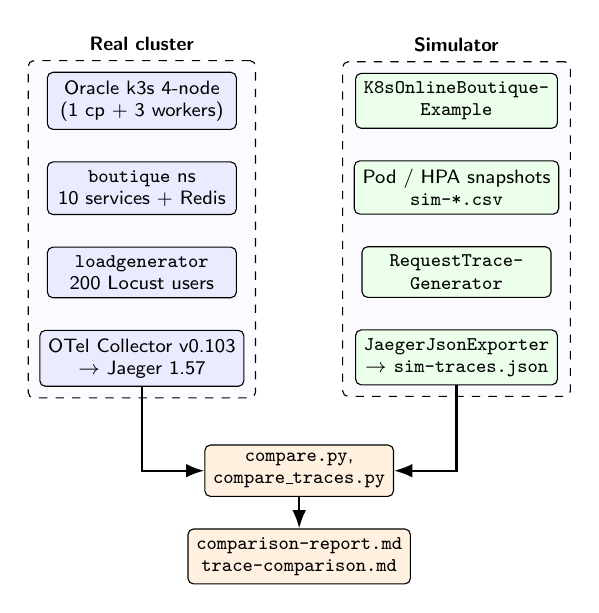
\begin{tikzpicture}[
            font=\scriptsize\sffamily,
            node distance=4mm and 5mm,
            real/.style={draw, rounded corners=2pt, fill=blue!8,
            inner sep=3pt, align=center, minimum width=24mm},
            sim/.style={draw, rounded corners=2pt, fill=green!8,
            inner sep=3pt, align=center, minimum width=24mm},
            cmp/.style={draw, rounded corners=2pt, fill=orange!12,
            inner sep=3pt, align=center, minimum width=22mm},
            pkg/.style={draw, dashed, rounded corners=2pt,
            inner sep=4pt, fill=blue!2},
            ar/.style={-Latex, thick}
        ]
% Real-side stack
            \node[real]                          (k3s)   {Oracle k3s 4-node\\(1 cp + 3 workers)};
            \node[real, below=of k3s]            (ns)    {\texttt{boutique} ns\\10 services + Redis};
            \node[real, below=of ns]             (lg)    {\texttt{loadgenerator}\\200 Locust users};
            \node[real, below=of lg]             (obs)   {OTel Collector v0.103\\$\to$ Jaeger 1.57};
% Two trace captures share this pipeline: USERS=200 (1020 traces,
% Table tab:boutique-results) and USERS=500 (1215 traces,
% deployment/online-boutique/runs/load500/trace-comparison.md).

% Simulator stack
            \node[sim, right=15mm of k3s]        (sim1)  {\texttt{K8sOnlineBoutique-}\\\texttt{Example}};
            \node[sim, below=of sim1]            (sim2)  {Pod / HPA snapshots\\\texttt{sim-*.csv}};
            \node[sim, below=of sim2]            (sim3)  {\texttt{RequestTrace-}\\\texttt{Generator}};
            \node[sim, below=of sim3]            (sim4)  {\texttt{JaegerJsonExporter}\\$\to$ \texttt{sim-traces.json}};

% Comparator
            \node[cmp, below=11mm of $(obs)!0.5!(sim4)$] (cmp) {\texttt{compare.py},\\\texttt{compare\_traces.py}};
            \node[cmp, below=of cmp]                    (rep) {\texttt{comparison-report.md}\\\texttt{trace-comparison.md}};

            \draw[ar] (obs.south) |- (cmp.west);
            \draw[ar] (sim4.south) |- (cmp.east);
            \draw[ar] (cmp) -- (rep);

% --- package framing boxes: drawn on the background layer so their fill
% never paints over the entity nodes above, regardless of source order ---
            \begin{pgfonlayer}{background}
            \node[fit=(k3s)(ns)(lg)(obs), pkg,
                label=above:{\textbf{Real cluster}}] (realbox) {};
            \node[fit=(sim1)(sim2)(sim3)(sim4), pkg,
                label=above:{\textbf{Simulator}}] (simbox) {};
            \end{pgfonlayer}
        \end{tikzpicture}
        \caption{Online Boutique paired validation pipeline.}
        \label{fig:boutique-topology}
    \end{figure}

    Unlike the synthetic RQ1--RQ4 sweeps, this track exercises the
    simulator against a production-grade polyglot workload that the
    broader CNCF community already runs in CI for upstream regressions,
    making the comparison self-validating for downstream researchers.

    \paragraph{Microservices architecture}
    Figure~\ref{fig:boutique-architecture} shows the boutique call graph
    that both substrates replay. The \texttt{frontend} accepts HTTP
    requests and fans out to nine downstream gRPC services written in five
    languages (Go, Python, Node.js, C\#, Java); \texttt{checkoutservice} in
    turn orchestrates the write path (shipping, payment, currency, email)
    and re-reads the cart and product catalogue. Orange nodes are the
    three HPA-managed services (\texttt{frontend}, \texttt{checkoutservice},
    \texttt{recommendationservice}, CPU target $70\%$); blue nodes are
    stateless gRPC backends; the grey node is the Redis cart store, and
    arrows denote synchronous gRPC calls. The graph is declared
    programmatically via \texttt{CallGraph} on the simulator side and is
    identical to the upstream \texttt{kubernetes-manifests.yaml v0.10.1}
    topology, so both substrates replay the same fan-out.

    \begin{figure*}[!t]
        \centering
        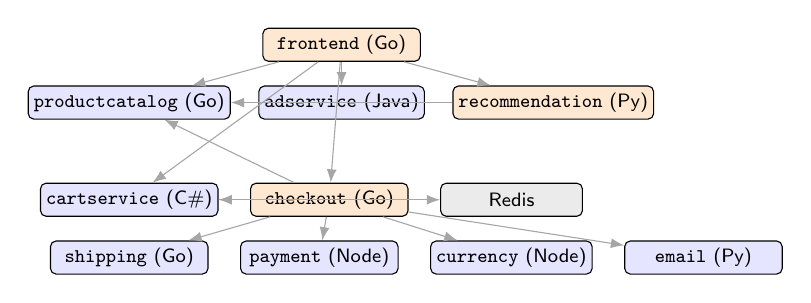
\begin{tikzpicture}[
            font=\scriptsize\sffamily,
            node distance=3mm and 4mm,
            svc/.style={draw, rounded corners=2pt, fill=blue!10,
            minimum height=4.2mm, minimum width=20mm,
            inner sep=2pt, align=center},
            hpa/.style={draw, rounded corners=2pt, fill=orange!18,
            minimum height=4.2mm, minimum width=20mm,
            inner sep=2pt, align=center},
            store/.style={draw, rounded corners=2pt, fill=black!8,
            minimum height=4.2mm, minimum width=18mm,
            inner sep=2pt, align=center},
            edge/.style={-Latex, thin, gray!70}
        ]
% top: frontend (HPA)
            \node[hpa]                                  (fe)   {\texttt{frontend} (Go)};
% second row: read-path
            \node[svc, below left=of fe]                (pc)   {\texttt{productcatalog} (Go)};
            \node[svc, below=of fe]                     (ad)   {\texttt{adservice} (Java)};
            \node[hpa, below right=of fe]               (rc)   {\texttt{recommendation} (Py)};
% third row: cart + checkout
            \node[svc, below=8mm of pc]                 (ca)   {\texttt{cartservice} (C\#)};
            \node[hpa, right=of ca]                     (co)   {\texttt{checkout} (Go)};
            \node[store, right=of co]                   (rd)   {Redis};
% fourth row: write-path leaves
            \node[svc, below=of ca]                     (sh)   {\texttt{shipping} (Go)};
            \node[svc, right=of sh]                     (pm)   {\texttt{payment} (Node)};
            \node[svc, right=of pm]                     (cu)   {\texttt{currency} (Node)};
            \node[svc, right=of cu]                     (em)   {\texttt{email} (Py)};
% fan-out from frontend
            \draw[edge] (fe) -- (pc);
            \draw[edge] (fe) -- (ad);
            \draw[edge] (fe) -- (rc);
            \draw[edge] (fe) -- (ca);
            \draw[edge] (fe) -- (co);
% recommendation fan-out
            \draw[edge] (rc) -- (pc);
% cart fan-out
            \draw[edge] (ca) -- (rd);
% checkout fan-out
            \draw[edge] (co) -- (sh);
            \draw[edge] (co) -- (pm);
            \draw[edge] (co) -- (cu);
            \draw[edge] (co) -- (em);
            \draw[edge] (co) -- (ca);
            \draw[edge] (co) -- (pc);
        \end{tikzpicture}
        \caption{Online Boutique call graph as replayed by the paired
        track.}
        \label{fig:boutique-architecture}
    \end{figure*}

    \paragraph{Distributed-tracing pipeline}
    A second validation axis compares simulated \emph{request traces}
    against traces emitted by the live cluster; the data flow is shown in
    Figure~\ref{fig:boutique-tracing}. On the real side (left),
    OpenTelemetry SDK instrumentation in each service exports spans over
    OTLP through the OpenTelemetry Collector into
    Jaeger~\cite{Jaeger2024,OpenTelemetry2024}, from which
    \texttt{pull\_jaeger\_traces.sh} materialises \texttt{real-traces.json}.
    On the simulator side (right), the tracing package walks the static
    \texttt{CallGraph} once per simulated request, drawing per-service
    service times from the \texttt{M/M/c} models (the same queueing module
    that powers RQ4), parameterised by the live container's CPU
    utilisation, and the \texttt{JaegerJsonExporter} writes
    \texttt{sim-traces.json}. Both branches emit Jaeger-v1-schema JSON that
    loads into the same UI without conversion; the comparator
    (\texttt{compare\_traces.py}) normalises operation names across the two
    sides and reports, per (service, op), the per-percentile latency and
    the symmetric ratio $\log_{10}(p95_\textrm{sim}/p95_\textrm{real})$
    (\texttt{trace-comparison.md}).

    \begin{figure}[!t]
        \centering
        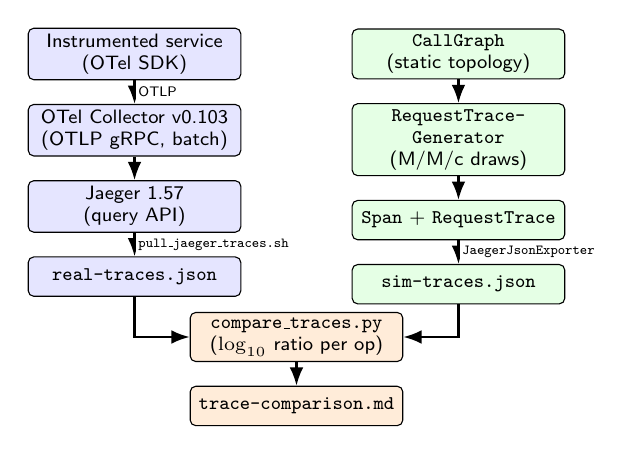
\begin{tikzpicture}[
            font=\scriptsize\sffamily,
            node distance=3mm and 5mm,
            real/.style={draw, rounded corners=2pt, fill=blue!10,
            minimum height=5mm, minimum width=27mm,
            inner sep=2pt, align=center},
            sim/.style={draw, rounded corners=2pt, fill=green!10,
            minimum height=5mm, minimum width=27mm,
            inner sep=2pt, align=center},
            cmp/.style={draw, rounded corners=2pt, fill=orange!15,
            minimum height=5mm, minimum width=27mm,
            inner sep=2pt, align=center},
            lbl/.style={font=\tiny\sffamily, fill=white, inner sep=1pt, align=center},
            ar/.style={-Latex, thick}
        ]
% real-side vertical flow
            \node[real]                       (svc)  {Instrumented service\\(OTel SDK)};
            \node[real, below=of svc]         (col)  {OTel Collector v0.103\\(OTLP gRPC, batch)};
            \node[real, below=of col]         (jg)   {Jaeger 1.57\\(query API)};
            \node[real, below=of jg]          (rj)   {\texttt{real-traces.json}};
% sim-side vertical flow
            \node[sim,  right=14mm of svc]    (cg)   {\texttt{CallGraph}\\(static topology)};
            \node[sim,  below=of cg]          (rg)   {\texttt{RequestTrace-}\\\texttt{Generator}\\(M/M/c draws)};
            \node[sim,  below=of rg]          (sp)   {\texttt{Span} + \texttt{RequestTrace}};
            \node[sim,  below=of sp]          (sj)   {\texttt{sim-traces.json}};
% comparator
            \node[cmp, below=4mm of $(rj)!0.5!(sj)$] (cmp) {\texttt{compare\_traces.py}\\($\log_{10}$ ratio per op)};
            \node[cmp, below=of cmp]                 (md)  {\texttt{trace-comparison.md}};

            \draw[ar] (svc) -- node[lbl,right]{OTLP} (col);
            \draw[ar] (col) -- (jg);
            \draw[ar] (jg)  -- node[lbl,right]{\texttt{pull\_jaeger\_traces.sh}} (rj);
            \draw[ar] (cg)  -- (rg);
            \draw[ar] (rg)  -- (sp);
            \draw[ar] (sp)  -- node[lbl,right]{\texttt{JaegerJsonExporter}} (sj);
            \draw[ar] (rj.south) |- (cmp.west);
            \draw[ar] (sj.south) |- (cmp.east);
            \draw[ar] (cmp) -- (md);
        \end{tikzpicture}
        \caption{Distributed-tracing pipeline: real cluster (left) vs.\
        simulator (right).}
        \label{fig:boutique-tracing}
    \end{figure}

    The trace study is a regime characterisation, not a fidelity claim: it
    delineates the load band over which the single-queue \texttt{M/M/c}
    approximation reproduces traced $p95$ latency and the band where its
    open-system assumption fails.
    Table~\ref{tab:boutique-results} summarises a ten-minute
    capture at $200$ concurrent Locust users under the moderate
    simulator profile, comprising $1{,}020$ real and $6{,}010$
    simulated traces. A second capture at \texttt{USERS=500},
    spanning a ten-minute window at $\approx\!95\,$RPS,
    drove the HPA to a non-degenerate plateau of six \texttt{frontend}
    pods, three \texttt{recommendationservice} pods, and one
    \texttt{checkoutservice} pod. The simulator under the calibrated
    high-load profile, with aggregate loads $3.80$, $1.80$, and $0.40$
    on the three elastic services, settles at the same plateau; the
    steady-state replica error is zero in all three cases. The per-pod
    load is supplied by a time-varying load model,
    $\textrm{CPU}_\textrm{pod}(t) = \min\!\big(\textrm{load}(t)/N(t),\,1\big)$,
    where $N(t)$ is the live replica count; the constant load-spreading
    used here is the special case $\textrm{load}(t){=}\textrm{const}$,
    and the same model (with ramp, step, spike, and sinusoidal curves)
    backs the interactive simulator's workload configuration. The
    full-trajectory un-aligned NRMSD values are $0.44$, $0.00$, and
    $0.77$ for frontend, checkoutservice, and recommendationservice
    respectively. To verify that this equilibrium is not an artefact of
    step-loading at $t{=}0$, a ramped-arrival variant (\texttt{high-ramp})
    drives the same three services from a low baseline up to the
    calibrated plateau over the first $180\,$s before holding: the HPA
    reaches the identical $6/3/1$ equilibrium, and the trajectory NRMSD
    is $0.47$, $0.00$, and $0.65$. The ramp does not lower the residual
    --- and marginally raises it for frontend --- because the real-side
    capture began after the HPA had already settled and so contains no
    transient to match (cf.\ footnote~g); the ramp's value is to confirm
    equilibrium robustness under a realistic arrival profile, not to
    improve the fit.
    Under saturation only \texttt{paymentservice/Charge} ($+0.21$)
    remains inside the $\pm 0.5$ acceptance band; the
    \texttt{ListRecommendations} order-of-magnitude match observed at USERS=200
    ($\log_{10}=-0.41$) does not survive at USERS=500
    ($\log_{10}=-1.36$). The real recommendation $p95$ rises from
    $46\,$ms at moderate load to $212\,$ms under saturation; the M/M/c
    approximation does not capture this throughput collapse and
    reports $p95 \approx 9.3\,$ms at the HPA equilibrium of three replicas
    ($\log_{10}(9.3 / 212) = -1.36$).
    Taken together, the two captures delineate the operating-regime
    envelope within which the single-queue M/M/c approximation holds.
    Figure~\ref{fig:boutique-trace-combined} plots both captures: each bar
    is one traced gRPC operation, the horizontal axis is the signed
    order-of-magnitude latency ratio $\log_{10}(p95_\textrm{sim} /
    p95_\textrm{real})$ (negative = simulator faster than real, positive =
    slower), and bars inside the shaded $\pm 0.5$ band are within the
    acceptance threshold for M/M/c order-of-magnitude agreement.
    \texttt{PlaceOrder} continues to drift in the sim-faster direction
    under saturation because the simulator span models only
    \texttt{checkoutservice}'s own service time rather than the
    orchestrating ten-service fan-out.

    \begin{figure}[!t]
        \centerline{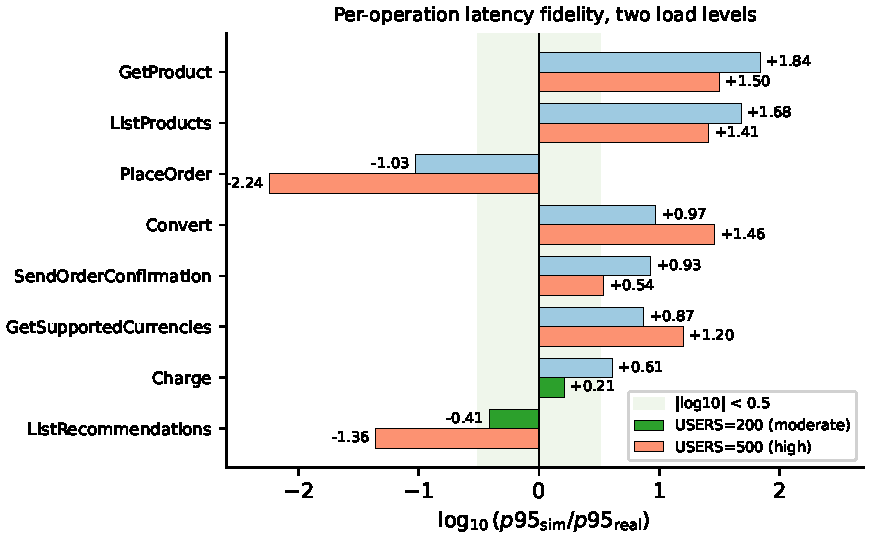
\includegraphics[width=\linewidth]{figures/boutique-trace-comparison-combined}}
        \caption{Per-operation $\log_{10}(p95_\textrm{sim} /
        p95_\textrm{real})$ at the two load levels (USERS=200, blue;
        USERS=500, red).}
        \label{fig:boutique-trace-combined}
    \end{figure}

    \paragraph{M/M/c regime envelope} At moderate load the per-elastic-pod
    CPU sits at $\approx\!70$--$85\%$ on the real cluster --- the M/M/c
    model's native operating regime --- and
    \texttt{ListRecommendations} achieves $\log_{10} = -0.41$ ($p95$
    of $17{,}875\,\mu$s vs.\ $46{,}383\,\mu$s real), the only operation
    within the $\pm 0.5$ band and evidence that the Erlang-C model captures
    queueing delay and service-time distribution to within an order of
    magnitude when the dominant operation is queue-limited. At
    saturation the same handler stops behaving like an Erlang-C queue
    and the M/M/c assumption becomes the dominant source of error.
    Catalog lookups and \texttt{PlaceOrder} diverge in the predicted
    asymmetric directions (sim slower on in-process hash-lookups, sim
    faster on cross-service fan-out spans) consistent with the
    simplifications documented in Section~\ref{sec:simplifications}.
    Placement and replica-count agreement (Table~\ref{tab:rq-results})
    hold across both load levels.

    \paragraph{Service-time characterisation} A per-operation analysis of
    the real gRPC spans
    quantifies \emph{why} the single-$\mu$ exponential service term bounds
    the approximation to the moderate regime, and motivates the
    M/M/c choice as a deliberate floor rather than a best fit. Two
    systematic departures from the $\textrm{Exp}(\mu)$ assumption appear.
    First, real service times are \emph{heavy-tailed}: the log-space
    standard deviation $\sigma$ of per-operation span durations ranges from
    $\approx\!0.4$ (e.g.\ \texttt{SendOrderConfirmation}) to $\approx\!2.3$
    (e.g.\ \texttt{GetCart} under load), and the coefficient of variation
    frequently exceeds the exponential's $\textrm{CV}=1$ --- so an
    M/G/c model with a lognormal service term would tighten the
    \emph{shape} match at a fixed load. Second, and more fundamentally,
    per-operation service time is \emph{load-dependent}: between USERS=200
    and USERS=500 the median span grows $2$--$9\times$
    (\texttt{paymentservice/Charge} $2.7\times$,
    \texttt{SendOrderConfirmation} $2.1\times$,
    \texttt{ListRecommendations} $6.8\times$, \texttt{PlaceOrder}
    $9.4\times$) as the production Go handlers degrade under contention.
    No fixed-distribution queue --- M/M/c or M/G/c --- can match both load
    levels simultaneously, because the service-time distribution itself
    shifts with utilisation; reproducing the saturation regime would
    require a load-dependent service model fitted to the captures, which
    we deliberately avoid as over-parameterisation. The single-queue
    Erlang-C model is therefore reported as a moderate-load,
    order-of-magnitude approximation with an empirically delimited regime
    boundary, not a universal latency predictor.

    \begin{table}[!t]
        \centering
        \caption{Per-operation latency at 200 Locust users (moderate sim
        profile): real Jaeger traces vs.\ \texttt{sim-traces.json} ($1{,}020$
        vs.\ $6{,}010$ traces). Status column is
            $\log_{10}(p95_\textrm{sim}/p95_\textrm{real})$;
            \checkmark{}~$=|\log|<0.5$.\label{tab:boutique-results}}
        \footnotesize
        \setlength{\tabcolsep}{3pt}
        \begin{tabular}{@{}lrrrrc@{}}
            \toprule
            & \multicolumn{2}{c}{\textbf{Real}\,($\mu$s)} & \multicolumn{2}{c}{\textbf{Sim}\,($\mu$s)} & \textbf{Ratio} \\
            \cmidrule(lr){2-3}\cmidrule(lr){4-5}
            \textbf{Operation}            & $p50$    & $p95$    & $p50$    & $p95$    & $\log_{10}$ \\
            \midrule
            \texttt{ListRecommendations}  & 5\,521   & 46\,383  & 4\,971   & 17\,875  & $-$0.41\,\checkmark \\
            \texttt{Charge}               & 367      & 1\,729   & 1\,716   & 7\,024   & $+$0.61 \\
            \texttt{GetSuppCurrencies}    & 114      & 1\,097   & 1\,744   & 8\,198   & $+$0.87 \\
            \texttt{SendOrderConfirm}     & 269      & 943      & 1\,645   & 7\,940   & $+$0.93 \\
            \texttt{Convert}              & 111      & 856      & 1\,845   & 8\,075   & $+$0.97 \\
            \texttt{PlaceOrder}           & 25\,239  & 63\,608  & 1\,422   & 5\,965   & $-$1.03 \\
            \texttt{ListProducts}         & 34       & 163      & 1\,795   & 7\,721   & $+$1.68 \\
            \texttt{GetProduct}           & 25       & 107      & 1\,741   & 7\,396   & $+$1.84 \\
            \bottomrule
        \end{tabular}
    \end{table}

%%============================================================
    \section{Discussion: Addressing Open Challenges from Prior Work}\label{sec:zarai-mapping}
%%============================================================

    Having established what \ckm models and validated it empirically, we
    now step back and relate the framework to the open research challenges
    that motivated it. A prior systematic review of intelligent autoscaling
    for cloud-native microservices~\cite{Zarai2025} flagged six
    future-direction themes across the surveyed literature. \ckm was not
    designed as a direct response to that review, but its architecture
    aligns with several of those themes; Table~\ref{tab:zarai-mapping} makes
    the alignment explicit so that researchers working along any of the six
    axes can identify the relevant extension points.

    \begin{table*}[!t]
        \centering
        \caption{Mapping from the six future-direction themes of
        Zarai2025~\cite{Zarai2025} to the features of \ckm that
        support research along each axis.\label{tab:zarai-mapping}}
        \begin{tabular*}{\textwidth}{@{\extracolsep{\fill}}p{0.30\textwidth}p{0.62\textwidth}@{}}
\toprule
\textbf{Future-direction theme~\cite{Zarai2025}} & \textbf{Alignment in \ckm} \\
\midrule
1. Adaptive and Proactive Learning &
The pluggable strategy interfaces of CloudSim Plus carry forward to
the Kubernetes layer: a custom \texttt{KubernetesScheduler} subclass or
\texttt{HorizontalPodAutoscaler} replacement can host an online or
federated-learning policy without modifying core framework code, as
demonstrated by the priority-class extensibility case study
(Section~\ref{sec:priority-case-study}). \\
\addlinespace
2. Workload- and System-Aware Modelling &
The PlanetLab trace driver exposes per-container CPU heterogeneity at
trace-sample fidelity;
microservice interdependencies are modelled via the
\texttt{services} package and \texttt{KubernetesService} call graphs;
heterogeneity across nodes is expressed through labels, taints, and
\texttt{NodeAffinity}. \\
\addlinespace
3. Advanced Forecasting and Policy Optimisation &
Tunable score blending (parameter $\lambda$),
asymmetric HPA stabilisation windows, and the eviction-style
preemption hook (Section~\ref{sec:priority-case-study}) provide the
extension points required to evaluate Transformer-, GNN-, or
hybrid-RL-driven scheduling and scaling decisions against deterministic
baselines. \\
\addlinespace
4. Comprehensive Resource and Cost Management &
Multi-resource accounting (CPU millicores, memory in MiB,
PE-level provisioning, bandwidth and storage from the CloudSim Plus
core); cost objectives via \texttt{VmAllocationPolicyTopologyAware}'s
\texttt{COST\_OPTIMIZED}/\texttt{LATENCY\_AWARE}/\texttt{SPREAD} modes;
PersistentVolume capacity accounting through \texttt{HarddriveStorage}. \\
\addlinespace
5. Operational Reliability and Real-world Deployment &
The documented simplifications of Section~\ref{sec:simplifications} make
the bounds of the simulator's validity an explicit contract rather than
implicit folklore; the asymmetric cooldown defaults ($300$\,s scale-down)
reproduce the operational guard-rails of production HPA.
External validation against a live cluster is
addressed by the companion artefact study (Section~\ref{sec:validation}). \\
\addlinespace
6. Security and Formal Guarantees &
\texttt{NetworkPolicy} ingress enforcement,
\texttt{ServiceAccount}/\texttt{Role}/\texttt{RoleBinding} metadata
registries, and the kubelet pre-flight that holds pods in
\texttt{Pending} until every declared dependency is registered enable
isolation and admission-control studies; the documented simplifications
explicitly delineate where formal guarantees do and do not hold. \\
\bottomrule
        \end{tabular*}
    \end{table*}

    The two themes that \ckm addresses most directly are themes~1
    and~3 (extension points for adaptive and advanced policies) and
    theme~5 (closing the sim-to-real gap through the explicit
    simplification contract). Themes~2 and~4 are supported via existing
    CloudSim Plus infrastructure surfaced into the Kubernetes layer.
    Theme~6 is partially supported by the security primitives; by the
    nature of a discrete-event simulator, formal proof of policy
    correctness is not provided, but the simulator offers a deterministic
    test bed in which such proofs can be empirically exercised.

%%============================================================
    \section{Conclusions}\label{sec:conclusions}
%%============================================================

    \ckm is a composition-based layer over CloudSim Plus (a minimal core
    footprint: one small \texttt{DatacenterSimple} edit plus
    \texttt{module-info} exports, no core logic changes) that models the
    Kubernetes orchestration stack under an explicit, test-enforced
    contract: every divergence from upstream Kubernetes is enumerated in
    Section~\ref{sec:simplifications}, paired with a regression test, and
    the validation gate treats any behaviour outside that list as a bug.
    The contract is the
    central engineering claim of the paper.

    The empirical results separate cleanly into three categories.
    \emph{Cross-tool fidelity} is the primary RQ1 result: scheduling
    decisions are agreement-checked against
    \texttt{kube-scheduler-simulator}~\cite{KubeSchSim2025}, which runs the
    production \texttt{kube-scheduler} binary on the identical 300-scenario
    set, under both deterministic and 5-run stochastic tie-breaks. This
    is a stronger comparator than any real-cluster check because it
    executes the exact upstream scheduling code path.
    \emph{Sim-to-real} validation on the 3-worker Oracle Cloud k3s
    substrate (with synthetic rack/zone labels) is reported in
    Table~\ref{tab:rq-results}: secondary RQ1 placement check, HPA
    trajectory and steady-state replica error (RQ2), VPA recommendation
    accuracy (RQ2b), and the Online Boutique paired track --- whose
    $\log_{10}=-0.41$ \texttt{ListRecommendations} match at moderate
    load (USERS=200) is the single best per-operation latency match
    ($1$ of $8$ traced operations within $\pm0.5\,\log_{10}$), reported
    as a best case rather than a universal latency-fidelity claim. A
    saturation-regime re-capture at USERS=500 establishes the
    operating-regime envelope: the match does not survive
    when the production Go gRPC handler queues beyond its modelled
    service capacity ($\log_{10} = -1.36$), so the M/M/c approximation
    is reported as a moderate-load fidelity claim rather than a
    universal one. The
    \emph{simulator-only} results are RQ3 scalability to 1{,}000 nodes
    (an algorithmic-complexity property of the event scheduler) and the
    Cluster Autoscaler round-trip; these do not imply sim-to-real
    fidelity at the corresponding scale and are clearly labelled as such
    throughout the manuscript. The constant-cost RQ4 proxy is reported
    only as a calibration check that the proxy never overestimates.

    The published simplifications list is itself the primary open work
    item: closing each entry is a unit of follow-up work that the
    contract makes individually addressable without breaking existing
    API consumers.

    Future work will extend the framework in several directions:
    resource quotas and limit ranges for namespace-scoped governance;
    custom-metrics HPA for memory- and request-rate-driven
    scaling~\cite{Li2023};
    PodDisruptionBudget-aware scale-down;
    VPA QoS-class reclassification side-effects;
    multi-cluster federation~\cite{Karmada2025};
    and reinforcement-learning scheduler plug-ins~\cite{Xie2024,Li2023}.
    The quantitative cross-comparison against
    \texttt{kube-scheduler-simulator}~\cite{KubeSchSim2025} on the RQ1
    scenario set --- previously listed as future work in early drafts ---
    is now part of the primary RQ1 evaluation
    (Section~\ref{sec:external-validation}); extending it to RQ2 (HPA
    trajectory) would require a Kubernetes simulator that also schedules
    arrival workloads, which is outside
    \texttt{kube-scheduler-simulator}'s scope.

    \ckm is offered as an open-source contribution to the
    \texttt{cloudsimplus/cloudsimplus} project and currently lives in a
    public development fork pending upstream review.\footnote{Fork
    carrying the \texttt{org.cloudsimplus.kubernetes} package:
    \url{https://github.com/Othmane-zarai/cloudsimplus-k8s}.} The Kubernetes
    extension ships inside the main CloudSim Plus artefact (no separate
    jar) and is consumed by importing from
    \texttt{org.cloudsimplus.kubernetes.*}. It builds against the
    in-development \texttt{org.cloudsimplus:cloudsimplus:9.0.0-SNAPSHOT}
    line; \emph{no 9.0.0 release is yet published to Maven Central}, where
    the latest public release is \texttt{8.5.7}. For reproducibility, the
    evaluation reported here was run on JDK~25.0.1 against the fork build.
    The exact snapshot is archived on Zenodo at
    \url{https://doi.org/10.5281/zenodo.21251757} (tag \texttt{v1.0.2},
    commit \texttt{172e2d9}).


%% --- Back matter ---
    \bmsubsection*{Author Contributions}
    Othmane Zarai: Conceptualization, Software, Writing---Original Draft,
    Writing---Review and Editing. Widad Ettazi: Supervision,
    Writing---Review and Editing. Riane Driss: Supervision, Writing---Review and Editing

    \bmsubsection*{Acknowledgments}
    The authors thank the CloudSim Plus development community for
    providing an extensible and well-documented simulation platform, and
    acknowledge the PlanetLab infrastructure for the CPU-utilisation traces
    that drive the PlanetLab worked example (\texttt{K8sPlanetLabExample}).
    During the preparation of this work, the authors used Claude
    (Anthropic), an AI-based coding assistant, to assist with LaTeX
    manuscript formatting and editorial restructuring (e.g.\ reorganising
    sections, tables, and figure captions). The authors reviewed and
    edited all AI-assisted content, verified it against the source
    materials and experimental results, and take full responsibility for
    the content of this publication.

    \bmsubsection*{Financial Disclosure}
    None reported.

    \bmsubsection*{Conflicts of Interest}
    The authors declare no conflicts of interest.

    \bmsubsection*{Data Availability Statement}
    The \texttt{org.cloudsimplus.kubernetes} extension that backs this paper
    lives in a public development fork of CloudSim Plus,
    \url{https://github.com/Othmane-zarai/cloudsimplus-k8s}, pending upstream
    review; it builds against the in-development
    \texttt{org.cloudsimplus:cloudsimplus:9.0.0-SNAPSHOT} line (the latest
    public release on Maven Central is \texttt{8.5.7}). The companion
    artefact for this paper --- the runnable Kubernetes examples, the headless
    CLI runner, the RQ1--RQ4 and Online Boutique deployment kit, the
    comparator scripts (\texttt{comparison-scripts/}), and the raw real-vs-sim
    captures --- is archived on Zenodo at
    \url{https://doi.org/10.5281/zenodo.21251747} (tag \texttt{v1.0.1},
    commit \texttt{7df3bb5}), while the \texttt{org.cloudsimplus.kubernetes}
    extension snapshot is archived at
    \url{https://doi.org/10.5281/zenodo.21251757} (tag \texttt{v1.0.2},
    commit \texttt{172e2d9}). The evaluation reported here was produced on
    JDK~25.0.1 against the fork build.

    \bibliography{kubernetes-refs}

\end{document}
